\documentclass[11pt,a4paper,openany]{book}

\usepackage[utf8]{inputenc}
\usepackage[T1]{fontenc}
\usepackage{lmodern}
\usepackage{amsmath,amssymb,amsthm}
\usepackage[margin=2.6cm]{geometry}
\usepackage{booktabs,array}
\usepackage{graphicx}
\usepackage{xcolor}
\usepackage{enumitem}
\usepackage{microtype}
\usepackage{listings}
\usepackage[most]{tcolorbox}
\usepackage{hyperref}
\hypersetup{colorlinks=true,linkcolor=black,urlcolor=blue!60!black,citecolor=black}


\DeclareUnicodeCharacter{1D4DD}{\ensuremath{\mathcal{N}}}
\DeclareUnicodeCharacter{211D}{\ensuremath{\mathbb{R}}}
\DeclareUnicodeCharacter{1DA0}{\ensuremath{^{f}}}
\makeatletter\def\verbatim@font{\footnotesize\ttfamily}\makeatother
\graphicspath{{figures/}}
\setlist{itemsep=2pt,topsep=4pt}

\newcommand{\Fzs}{F_0^{s}}
\newcommand{\Fos}{F_1^{s}}
\newcommand{\code}[1]{\texttt{\hyphenchar\font=`\-\relax #1}}
\newcommand{\Q}{\mathbb{Q}}
\newcommand{\R}{\mathbb{R}}

% ---------------------------------------------------------------- boxes
\definecolor{runbg}{HTML}{EEF4FB}
\definecolor{runframe}{HTML}{2A78D6}
\definecolor{objbg}{HTML}{F4F4F1}
\definecolor{warnbg}{HTML}{FBF1EA}
\definecolor{warnframe}{HTML}{EB6834}

\newtcolorbox{runit}{breakable,colback=runbg,colframe=runframe,boxrule=0.6pt,arc=2pt,
  left=6pt,right=6pt,top=4pt,bottom=4pt,fonttitle=\bfseries\small,title={Run it yourself}}
\newtcolorbox{objectives}{colback=objbg,colframe=black!45,boxrule=0.4pt,arc=2pt,
  left=6pt,right=6pt,top=4pt,bottom=4pt,fonttitle=\bfseries\small,title={Learning objectives}}
\newtcolorbox{lesson}[1][]{breakable,colback=warnbg,colframe=warnframe,boxrule=0.6pt,arc=2pt,
  left=6pt,right=6pt,top=4pt,bottom=4pt,fonttitle=\bfseries\small,title={#1}}

% ---------------------------------------------------------------- theorem-like environments
\theoremstyle{definition}
\newtheorem{definition}{Definition}[chapter]
\newtheorem{example}{Worked example}[chapter]
\newtheorem{exercise}{Exercise}[chapter]
\theoremstyle{plain}
\newtheorem{theorem}{Theorem}[chapter]
\newtheorem{proposition}[theorem]{Proposition}

% ---------------------------------------------------------------- code listings
\lstset{basicstyle=\ttfamily\small,columns=fullflexible,keepspaces=true,breaklines=true,
  frame=single,rulecolor=\color{black!30},xleftmargin=4pt,xrightmargin=4pt,
  extendedchars=true,
  literate={ℝ}{{$\mathbb{R}$}}1 {≤}{{$\le$}}1 {→}{{$\to$}}1 {∧}{{$\wedge$}}1
           {⟨}{{$\langle$}}1 {⟩}{{$\rangle$}}1 {‖}{{$\Vert$}}1 {⁻¹}{{$^{-1}$}}2
           {ᶠ}{{$^{f}$}}1 {∀}{{$\forall$}}1 {𝓝}{{$\mathcal{N}$}}1 {·}{{$\cdot$}}1
           {₀}{{$_0$}}1 {∫}{{$\int$}}1 {≃}{{$\simeq$}}1 {⁽}{{$^($}}1 {⁾}{{$^)$}}1 {¹}{{$^1$}}1}

\title{\textbf{Exact Kinetic Theory with a Proof Assistant}\\[6pt]
\large A training guide and textbook built on the SocrateAI Agora engine\\[4pt]
\normalsize Zero sound, Padé approximants over $\Q$, Villani's Theorem~22.6,\\
helium data, Lean~4, and how to contribute as a scientist or an AI agent}
\author{Xavier Callens\\ \textit{Laboratoire SocrateAI, Cagnes-sur-Mer, France}}
\date{First edition, 27 September 2026}

\begin{document}
\sloppy
\frontmatter
\maketitle

\chapter*{Preface}
\addcontentsline{toc}{chapter}{Preface}

This book teaches a way of doing theoretical physics with a computer in which every claim is
backed by something that would fail if the claim were false. It is built around one open-source
repository, \emph{SocrateAI-Scientific-Agora-Physique-Cinetique}, and every number in it comes
from that repository: from its test suite, from committed result files under
\code{alexandrie\_data/}, from its verification scripts, or from its research paper
\code{docs/agora\_engine\_paper.pdf}. Where a chapter quotes a number, a box nearby tells you the
command that reproduces it.

The book is meant for three kinds of reader.
\begin{itemize}
  \item \textbf{Students} in physics, mathematics or computer science, at the level of an advanced
        undergraduate or beginning graduate course. You should know calculus, linear algebra, a
        little complex analysis and basic Python. Statistical mechanics helps but is not required.
  \item \textbf{Researchers} who want to see what exact arithmetic and a proof assistant can and
        cannot contribute to kinetic theory and quantum fluids.
  \item \textbf{AI coding agents} (Claude Code, Google Jules and others) and the people who direct
        them. Part~II explains the conventions an agent must follow to contribute, and why they
        exist.
\end{itemize}

\paragraph{The honesty rule.} This project has withdrawn several of its own earlier claims. The
withdrawals are recorded in \code{RETRACTIONS.md} (entries R1--R9), and this book uses them as
teaching material, because each one shows a specific way that fluent, confident output, produced
by a person or a model, can be wrong. A chapter that presents a result also says what it does
\emph{not} show. Numerical evidence is never called a proof. A Lean theorem proves a statement
about a mathematical model, never by itself a statement about real helium.

\paragraph{How to use this book.} Part~I (Chapters~\ref{ch:exact}--\ref{ch:phasemixing}) is the
theory; read it in order. Part~II (Chapters~\ref{ch:engine}--\ref{ch:contrib}) is practice and can
be read selectively. Each chapter opens with learning objectives and ends with exercises; solutions
are in Appendix~\ref{app:solutions}. ``Run it yourself'' boxes give exact shell commands, to be
run from the repository root after
\begin{verbatim}
git clone https://github.com/xaviercallens/SocrateAI-Scientific-Agora-Physique-Cinetique
cd SocrateAI-Scientific-Agora-Physique-Cinetique
pip install -r requirements.txt
export PYTEST_DISABLE_PLUGIN_AUTOLOAD=1   # avoids unrelated global pytest plugins
\end{verbatim}

\paragraph{Evidence levels.} Throughout, claims are labelled by the evidence behind them:
\begin{description}[leftmargin=2.2em,style=nextline]
  \item[Level 1] exact symbolic computation over $\Q$ (or exact algebraic numbers);
  \item[Level 2] independent numerical validation, e.g.\ 60-digit root finding or a separate
        implementation in another language;
  \item[Level 3] a machine-checked proof in Lean~4 with Mathlib, audited with \code{\#print axioms};
  \item[Level 4] comparison with published experimental data.
\end{description}
The research paper groups the data checks with Level~2; this book separates them, because
confronting a model with measurement is a different act from checking its arithmetic.

\tableofcontents

\mainmatter

%==========================================================================================
\part{Foundations}
%==========================================================================================

%------------------------------------------------------------------------------------------
\chapter{Why exact arithmetic}
\label{ch:exact}
%------------------------------------------------------------------------------------------

\begin{objectives}
After this chapter you should be able to
\begin{itemize}
  \item name two distinct ways machine-assisted physics fails, and the defence against each;
  \item explain what the ``Z\'ero Simulation Flottante'' rule forbids and what it allows;
  \item say precisely what ``verified'' means at each evidence level, and what it does not mean.
\end{itemize}
\end{objectives}

\section{Two failure modes}

The first failure mode is recent. A language model asked for a derivation can produce fluent,
well-formatted mathematics that is wrong, and the error is hard to see precisely because the
output looks like the real thing. The same is true of an automated \emph{audit}: this project
contains an audit report, written by an automated pass, that described repairs as complete before
they were made (\code{RETRACTIONS.md}, R6). Among its claims were that two coefficient tables had
been unified while one of the files was untouched, and that a feature was ``fully implemented''
while the code passed a polynomial into a function expecting a list of Taylor coefficients.

The second failure mode is older. A continuous kinetic problem discretised into 64-bit floating
point loses, irrecoverably, the analytic structure that governs its qualitative behaviour. Phase
mixing, Landau damping and the location of collective modes depend on branch points and on exact
cancellations. A floating-point pipeline reports these as small residuals, and a small residual
looks the same whether it is a rounding artefact or physics.

The defence against both is the same, and it is the organising principle of this book:
\begin{quote}
\emph{A claim is only as good as the executable check that would fail if the claim were false.}
\end{quote}
Prose, however careful, is not such a check. A test that re-derives a coefficient from its closed
form is. So is a proof that the Lean kernel accepts, and so is a comparison with a published
measurement.

\section{The rule: no floating point in a derivation}

The engine represents every quantity that enters a derivation exactly. Series coefficients are
rational numbers (\code{sympy.Rational}); approximants are obtained by exact linear algebra over
$\Q$; dispersion relations become polynomials with rational coefficients; their roots are
algebraic numbers, returned in closed form or with their minimal polynomial.

Floating point is not banned from the project. It is \emph{quarantined}. It appears in
\code{verification/}, \code{simulations/} and \code{notebooks/}, and only to check an exact
result against an independent reference, never to produce the result being checked. The
direction matters: an exact result certifies a numerical computation, never the reverse.

\subsection{Enforced, not documented}

A rule that nothing checks is a comment. Three mechanisms make this rule operative.

\paragraph{Refusal at the boundary.} Entry points that accept a physical parameter reject
floating-point input. Passing $\Fzs$ as the Python float \code{9.3} raises
\code{ScientificHonestyException} rather than silently converting it. The test
\code{test\_float\_coupling\_is\_refused} keeps this true. The rule was added after an earlier
revision did exactly the dangerous thing: it wrote
\code{sp.Rational(float(F0s)).limit\_denominator(1000)}, a round trip that can change the very
parameter whose exactness is the point (R6).

\paragraph{Exact representation end to end.} Stored results contain strings such as
\code{13265/11482 - 5*sqrt(4144945)/11482}, not decimals.

\paragraph{Identities tested against closed forms, not tables.} A hard-coded coefficient table is
indistinguishable from a fabricated one. The test suite therefore re-derives kernel coefficients
from the closed-form generating function symbolically and compares
(\code{test\_landau\_kernel\_matches\_closed\_form}). A table typed in by hand, or produced by a
model, fails the test unless it is right.

\begin{example}[Why $0.1$ is not $1/10$]
In binary floating point, $0.1$ is stored as the nearest dyadic rational,
\[
  \texttt{float(0.1)} = \frac{3602879701896397}{36028797018963968},
\]
which is not $1/10$. In sympy, \code{Rational(0.1)} returns that dyadic number, while
\code{Rational("0.1")} and \code{Rational(1,10)} return $1/10$. This is why every interface of
the engine, including the MCP server of Chapter~\ref{ch:mcp}, accepts numbers as \emph{strings}
or fractions and refuses Python floats.
\end{example}

\section{What ``verified'' means, and does not}

The word ``verified'' has been over-used in this project's history, and learning to use it
precisely is part of the training.
\begin{itemize}
  \item A Level~1 computation shows that an algebraic manipulation is correct. It says nothing about
        whether the model being manipulated describes nature.
  \item A Level~2 validation shows that an exact result agrees with an independent computation of
        the same mathematical object.
  \item A Level~3 proof shows that a mathematical statement follows from Mathlib's axioms. The
        early Lean file of this project proved, among other things, $2\cdot2=4$ after unfolding a
        definition, and a theorem whose hypothesis was its conclusion (R3). Both compiled. Both
        are ``verified''. Neither says anything about physics.
  \item A Level~4 comparison with data can falsify a model. Chapter~\ref{ch:data} shows it doing
        exactly that.
\end{itemize}

\begin{lesson}[Lesson from the retractions: grep is not a proof audit]
The absence of the string \code{sorry} in a Lean file does not show that its theorems are
proved: a theorem can depend on \code{sorryAx} through an import. The project therefore ends every
Lean file with \code{\#print axioms} for each theorem, and continuous integration fails if
\code{sorryAx} appears in the output (Chapter~\ref{ch:lean}).
\end{lesson}

\begin{runit}
\begin{verbatim}
python3 -m pytest tests/ -q          # 49 tests, including the float-refusal test
python3 -c "import sympy as sp; print(sp.Rational(0.1), sp.Rational('0.1'))"
\end{verbatim}
\end{runit}

\section*{Exercises}
\begin{exercise}\label{ex:float-roundtrip}
Let $F=1/1001$. Compute \code{Rational(float(F)).limit\_denominator(1000)} by hand or in
Python. What went wrong, and why is this worse than a rounding error in the tenth digit?
\end{exercise}
\begin{exercise}\label{ex:levels}
Classify each statement by evidence level (1--4), or say that it has none:
(a) ``the $[1/1]$ Padé root at $\Fzs=93/10$ is $u=10/37$'';
(b) ``the $[4/4]$ root agrees with a 60-digit solution to $6.8\times10^{-10}$'';
(c) ``every undamped zero-sound root satisfies $s-1\le\Fzs$'';
(d) ``in liquid $^3$He zero sound is faster than first sound at 0~bar'';
(e) ``this kernel protects 2D quantum films from Landau damping collapse''.
\end{exercise}
\begin{exercise}\label{ex:tabletest}
Explain why a test comparing code output with a hard-coded table of coefficients cannot detect a
fabricated table, while a test that re-derives the coefficients from a closed form can.
\end{exercise}

%------------------------------------------------------------------------------------------
\chapter{Power series and Padé approximants over \texorpdfstring{$\mathbb{Q}$}{Q}}
\label{ch:pade}
%------------------------------------------------------------------------------------------

\begin{objectives}
\begin{itemize}
  \item construct a diagonal $[M/M]$ Padé approximant from Taylor coefficients by exact linear
        algebra;
  \item understand why a Padé approximant can succeed where a truncated series fails, and where
        it must fail;
  \item turn a transcendental equation into a polynomial one over $\Q$.
\end{itemize}
\end{objectives}

\section{From a series to a rational function}

Let $A(u)=\sum_{n\ge0}a_nu^n$ with rational $a_n$. A truncated Taylor polynomial of degree $2M$
uses $2M+1$ coefficients. A \emph{diagonal Padé approximant} $[M/M]$ uses the same coefficients to
build a ratio of two polynomials of degree $M$,
\begin{equation}
  \frac{P(u)}{Q(u)}, \qquad Q(0)=1,
\end{equation}
fixed by the requirement that it agree with $A$ to the same order:
\begin{equation}
  A(u)\,Q(u) - P(u) = \mathcal{O}\!\left(u^{2M+1}\right).
  \label{eq:padeorder}
\end{equation}
Write $Q(u)=1+\sum_{j=1}^M q_ju^j$ and $P(u)=\sum_{j=0}^M p_ju^j$. The coefficient of $u^n$ in
$AQ-P$ is $a_n+\sum_{j=1}^{\min(n,M)}q_ja_{n-j}-p_n$ (with $p_n=0$ for $n>M$). The conditions
split into two groups.
\begin{itemize}
  \item For $n=M+1,\dots,2M$, $p_n=0$, and the conditions form an $M\times M$ linear system for
        $q_1,\dots,q_M$ whose matrix is a Hankel matrix of the $a_n$.
  \item For $n=0,\dots,M$, the conditions give $p_n$ directly once the $q_j$ are known.
\end{itemize}
Every step is exact over $\Q$. The engine's \code{KineticStage.pade\_diagonal} does precisely this
and \emph{refuses} to return an approximant if the Hankel system is singular, instead of falling
back on a least-squares surrogate.

\begin{example}[{The $[1/1]$ approximant of the zero-sound kernel}]
\label{ex:pade11}
Chapter~\ref{ch:zerosound} shows that the kernel we care about has $a_0=0$ and
$a_k=1/(2k+1)$ for $k\ge1$, so $a_1=1/3$, $a_2=1/5$. With $M=1$ the single condition for $n=2$ is
\[
  a_2+q_1a_1=0 \;\Longrightarrow\; \tfrac15+\tfrac{q_1}{3}=0 \;\Longrightarrow\; q_1=-\tfrac35 .
\]
The conditions for $n=0,1$ give $p_0=a_0=0$ and $p_1=a_1+q_1a_0=1/3$. Hence
\begin{equation}
  P(u)=\frac u3,\qquad Q(u)=1-\frac{3u}{5}.
  \label{eq:pade11}
\end{equation}
This order condition is one of the identities machine-checked in \code{Protocols.lean}. It has
content: it is the equation that \emph{determines} $q_1$, not a restatement of its definition.
\end{example}

\begin{example}[{The $[2/2]$ approximant}]
Solving the $2\times2$ Hankel system with $a_1,\dots,a_4=1/3,1/5,1/7,1/9$ gives, exactly,
\[
  P(u)=\frac u3-\frac{23u^2}{135},\qquad Q(u)=1-\frac{10u}{9}+\frac{5u^2}{21}.
\]
You will verify this in Exercise~\ref{ex:pade22}.
\end{example}

\section{Why Padé, and where it fails}

A truncated power series is a polynomial and cannot have a singularity. A rational function can
have poles, so a Padé approximant can mimic a function that has a pole or, less perfectly, a branch
point. For functions of Stieltjes type, whose singularities lie on a cut, diagonal Padé
approximants converge away from the cut, and their poles accumulate along it
\cite{bakergravesmorris}. This is the good news: at strong coupling the zero-sound root lies far
from the cut and the approximants converge geometrically (Chapter~\ref{ch:zerosound}).

The bad news is structural. A logarithmic branch point cannot be represented by finitely many
poles. Close to it, any finite-order approximant built from the expansion at $u=0$ is wrong in a
way that no increase of order repairs quickly. Chapter~\ref{ch:zerosound} shows that this is
exactly where the weak-coupling zero-sound mode lives, and that the method therefore fails there.
That failure is a result and is tested as such.

\section{From a transcendental equation to a polynomial}

Suppose the physics asks for a root of $A(u)=c$ with $c\in\Q$. Replacing $A$ by $P/Q$ gives
\[
  P(u)-c\,Q(u)=0,
\]
a polynomial equation with rational coefficients. Its roots are algebraic numbers: degree~1 roots
are rationals, degree~2 roots involve one square root, and higher degrees are represented by the
polynomial and an index (sympy's \code{CRootOf}). The engine returns them in that form, which is
the form a proof assistant can consume.

\begin{runit}
\begin{verbatim}
python3 -c "
from agora_swarm.agents.linear_response import LinearResponseStage
from agora_swarm.agents.kinetic import KineticStage
a = LinearResponseStage().landau_zero_sound_kernel(order=6)
P, Q, u = KineticStage().pade_diagonal(a, 2)
print(P, '|', Q)"
python3 -m pytest tests/test_protocols.py -q -k pade
\end{verbatim}
\end{runit}

\section*{Exercises}
\begin{exercise}\label{ex:padeexp}
Construct the $[1/1]$ Padé approximant of $e^x$ and compare its value at $x=1$ with $e$ and with
the Taylor polynomial $1+x+x^2/2$.
\end{exercise}
\begin{exercise}\label{ex:pade22}
Write out the $2\times2$ Hankel system for the $[2/2]$ approximant of $\sum_{k\ge1}u^k/(2k+1)$,
solve it over $\Q$, and check the $P$ and $Q$ given above.
\end{exercise}
\begin{exercise}\label{ex:singular}
Give a series for which the $[1/1]$ Hankel system is singular. What should an exact engine do in
that case, and why is a least-squares fallback dangerous here?
\end{exercise}

%------------------------------------------------------------------------------------------
\chapter{Landau Fermi liquids and zero sound}
\label{ch:zerosound}
%------------------------------------------------------------------------------------------

\begin{objectives}
\begin{itemize}
  \item derive the zero-sound kernel and its rational Taylor coefficients;
  \item solve the one-parameter dispersion relation exactly with Padé approximants and judge the
        result against a 60-digit reference;
  \item state and interpret the weak-coupling bracket, a theorem proved in Lean;
  \item extend the model to two Landau parameters and keep the computation exact.
\end{itemize}
\end{objectives}

\section{Collisionless sound in a Fermi liquid}

At low temperature, liquid $^3$He is a Fermi liquid: its low-energy excitations are quasiparticles
near a Fermi surface of radius $k_F$, with Fermi velocity $v_F$ and effective mass $m^*$. Their
interaction is described by Landau parameters $F_l^s$, $F_l^a$, the Legendre components of the
spin-symmetric and antisymmetric interaction \cite{pinesnozieres}.

When collisions are frequent, sound is ordinary hydrodynamic \emph{first sound}, with speed $c_1$.
At frequencies above the collision rate there is a different, collisionless mode, \emph{zero
sound}, a coherent deformation of the Fermi surface. Landau predicted it, and it was observed in
$^3$He in the 1960s. Write its speed as $c_0=s\,v_F$. The dimensionless velocity $s$ is fixed by a
dispersion relation derived from the linearised Landau kinetic equation.

\section{The kernel and its coefficients}

Keeping only the $l=0$ parameter $\Fzs$, the dispersion relation is
\begin{equation}
  \chi(s)=\frac{1}{\Fzs},\qquad
  \chi(s)=\frac s2\ln\frac{s+1}{s-1}-1,\qquad s=\frac{\omega}{qv_F}.
  \label{eq:disp}
\end{equation}
An \emph{undamped} mode needs $s>1$: its phase velocity must exceed every quasiparticle velocity,
otherwise it would resonate with quasiparticles and decay (Landau damping). The region $s<1$ is the
particle--hole continuum.

Put $u=1/s^2$. Since $\frac s2\ln\frac{s+1}{s-1}=s\,\operatorname{artanh}(1/s)$ and
$\operatorname{artanh}x=\sum_{k\ge0}x^{2k+1}/(2k+1)$,
\begin{equation}
  \chi=\sum_{k\ge1}a_ku^k,\qquad \boxed{\,a_k=\frac1{2k+1}\,}.
  \label{eq:ak}
\end{equation}
All coefficients are rational. The test \code{test\_landau\_kernel\_matches\_closed\_form}
re-derives them symbolically from \eqref{eq:disp}.

\begin{lesson}[Lesson from the retractions: two kernels, one name]
Earlier revisions used the name ``Lindhard'' for two different functions, and the repository came
to contain three mutually inconsistent coefficient tables: $1/3,\,19/45$ in Lean,
$2/3,\,2/15$ in Python, and $1/(2k+1)$ in the prose (R4). The resolution is that $1/(2k+1)$ is
correct for the zero-sound kernel; the sequence $2/(4k^2-1)$ belongs to a different function,
$g(x)=1+\frac{x^2-1}{2x}\ln\frac{1+x}{1-x}$, kept under the name \code{legacy\_algebraic\_kernel};
and $19/45$ corresponded to neither. A test now asserts that the two sequences differ, so they
cannot be conflated again.
\end{lesson}

\section{The exact solution}

With $\chi\approx P/Q$, Eq.~\eqref{eq:disp} becomes the polynomial equation
\begin{equation}
  Q(u)-\Fzs P(u)=0,\qquad\text{admissible roots } u\in(0,1).
  \label{eq:disppoly}
\end{equation}
At $M=1$, Eq.~\eqref{eq:pade11} gives the closed form
\begin{equation}
  u=\frac{15}{9+5\Fzs}.
  \label{eq:root11}
\end{equation}

\begin{example}[A $^3$He-like coupling]
For the stand-in value $\Fzs=93/10$, Eq.~\eqref{eq:root11} gives $u=15/(9+93/2)=10/37$ and
\[
  s=\sqrt{37/10}=1.923538406167134\ldots
\]
At higher order the roots are algebraic numbers of degree 2, 3 and 4 (Table~\ref{tab:exact}).
\end{example}

\begin{table}[htbp]
\centering
\caption{Exact admissible roots $u$ of Eq.~\eqref{eq:disppoly} returned by the engine
(\code{docs/agora\_engine\_paper.pdf}, Table~1). $\mathrm{CRootOf}(p,0)$ is the first real root
of $p$.}
\label{tab:exact}
\small
\begin{tabular}{ll>{\raggedright\arraybackslash}p{9.6cm}}
\toprule
$\Fzs$ & $M$ & exact admissible root $u$ \\
\midrule
$93/10$ & 1 & $10/37$ \\
$93/10$ & 2 & $13265/11482 - 5\sqrt{4144945}/11482$ \\
$93/10$ & 3 & $\mathrm{CRootOf}(102367u^{3} - 582876u^{2} + 708015u - 150150,\,0)$ \\
$30$ & 1 & $5/53$ \\
$30$ & 2 & $350/337 - \sqrt{101269}/337$ \\
$1$ & 1 & none in $(0,1)$ \\
$1$ & 2 & $1365/772 - 3\sqrt{44905}/772$ \\
\bottomrule
\end{tabular}
\end{table}

\subsection{Judging the result}

The exact roots solve the \emph{approximate} equation. How good is the approximation? The
verification script solves the transcendental equation \eqref{eq:disp} to 60 digits with
\code{mpmath} and compares (Level~2). This is the only place floating point enters, and it is
outside the derivation. Figure~\ref{fig:pade} shows the result. At strong coupling the convergence
is geometric: $6.8\times10^{-10}$ at $M=4$ for $\Fzs=93/10$, and $7.7\times10^{-14}$ for
$\Fzs=30$. At $\Fzs=1$ it is slow, and at $\Fzs=1/2$ and $1/10$ there is no admissible root at
any order tested.

\begin{figure}[htbp]
\centering
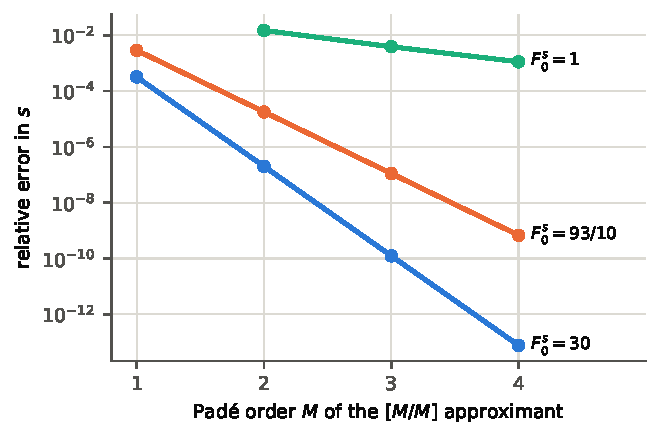
\includegraphics[width=0.72\textwidth]{pade_convergence.pdf}
\caption{Relative error of the exact Padé root against the 60-digit solution of
Eq.~\eqref{eq:disp}, from Table~2 of the engine paper. At $\Fzs=1$ the $M=1$ approximant has no
admissible root.}
\label{fig:pade}
\end{figure}

\section{Weak coupling: a negative result and a theorem}

Why does the method fail at weak coupling? At $M=1$, Eq.~\eqref{eq:root11} gives $u>1$ as soon as
$\Fzs<6/5$, and higher orders do not repair this. The reason is the branch point of $\chi$ at
$s=1$, that is at $u=1$, the edge of the continuum. As $\Fzs\to0^+$ the true root approaches the
branch point according to
\begin{equation}
  s-1\;\simeq\;2e^{-2-2/\Fzs},
  \label{eq:threshold}
\end{equation}
exponentially close, and a finite set of poles cannot resolve a logarithm at exponentially small
distance. The engine reports \code{root\_found: false} with a reason, and a test asserts that it
continues to do so, so that a future change cannot quietly return a spurious root.

\begin{lesson}[Lesson from the retractions: a capability that never existed]
The protocol registry once promised to track ``the velocity ratio drop $v_{zs}\le v_F$ into the
Landau damping continuum'' with rational Padé approximants. That is unattainable by this
construction, and no implementation of it ever existed (R6, R7). The negative result above replaced
the promise.
\end{lesson}

Is the mode really there when the method cannot find it? Yes, and this is now a theorem. Write
$g_3(s)=\chi(s)$ as a function of $s>1$. Two elementary bounds on the logarithm give
\[
  \tfrac12\ln\frac{2}{s-1}-1\;\le\;g_3(s)\;\le\;\frac1{s-1}.
\]
Evaluating both at a root, where $g_3(s)=1/\Fzs$, gives:

\begin{theorem}[Zero-sound bracket; \code{zero\_sound\_bracket} in \code{ZeroSoundBracket.lean}]
\label{thm:bracket}
If $\Fzs>0$, $s>1$ and $g_3(s)=1/\Fzs$, then
\begin{equation}
  2e^{-(2+2/\Fzs)}\;\le\;s-1\;\le\;\Fzs .
  \label{eq:bracket}
\end{equation}
\end{theorem}

This is proved over $\R$ in Lean~4 with Mathlib (Level~3). A companion project proves that such a
root exists for every $\Fzs>0$. Two consequences follow. First, the lower edge is exactly the
asymptotic law \eqref{eq:threshold}, and the numerics show that it is attained as $\Fzs\to0$: the
ratio $(s-1)/(2e^{-2-2/\Fzs})$ is $1.0000000$ at $\Fzs=1/20$ and $1/10$, $1.0000069$ at $3/20$
and $1.0031716$ at $3/10$. The proved bound is asymptotically sharp. Second, since the root exists,
the Padé failure is a limitation of the \emph{method}, not an absence of the mode.
Figure~\ref{fig:bracket} shows the bracket with the 60-digit roots.

\begin{figure}[htbp]
\centering
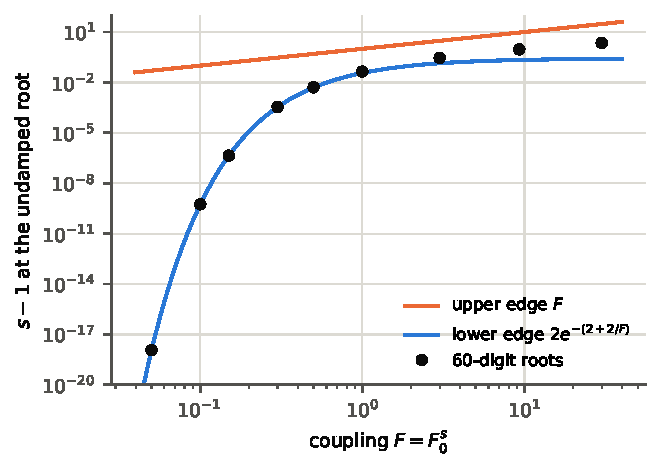
\includegraphics[width=0.72\textwidth]{zero_sound_bracket.pdf}
\caption{The proved bracket \eqref{eq:bracket} and the 60-digit roots of Eq.~\eqref{eq:disp},
recomputed by \code{docs/textbook/figures/make\_figures.py}. The lower edge hugs the roots at
weak coupling.}
\label{fig:bracket}
\end{figure}

\section{Two Landau parameters}

The value $\Fzs=93/10$ was a stand-in. Chapter~\ref{ch:data} uses real $^3$He parameters and
shows that the one-parameter model is then wrong: it puts zero sound below first sound. The fix
is the $l=1$ parameter $\Fos=3(m^*/m-1)$, which couples density to current. With it the
dispersion relation becomes
\begin{equation}
  g_3(s)=\frac1{\tilde F(s)},\qquad \tilde F(s)=\Fzs+\frac{\Fos s^2}{1+\Fos/3}.
  \label{eq:f0f1}
\end{equation}
The verification script does not take this on trust: it checks it against a direct solution of
the $l=0,1$ moment equations of the Landau kinetic equation, a $2\times2$ determinant with moments
computed by quadrature.

The exact method carries over. With $u=1/s^2$, $a=1+\Fos/3$ and $\chi\approx P/Q$,
Eq.~\eqref{eq:f0f1} becomes
\begin{equation}
  P(u)\,(\Fzs au+\Fos)-Q(u)\,au=0,
  \label{eq:f0f1poly}
\end{equation}
again a polynomial over $\Q$, implemented as \code{solve\_zero\_sound\_root\_f0\_f1}. The first
sound speed follows from the same parameters,
\begin{equation}
  c_1=v_F\sqrt{\frac{(1+\Fzs)(1+\Fos/3)}{3}}.
  \label{eq:c1}
\end{equation}

\begin{runit}
\begin{verbatim}
python3 simulations/qv_01_zero_sound.py        # exact QV-01 derivation
python3 verification/validate_zero_sound.py    # 60-digit check, asserts the bracket
python3 -m pytest tests/test_protocols.py -q -k "zero_sound"
\end{verbatim}
\end{runit}

\section*{Exercises}
\begin{exercise}\label{ex:ak}
Derive $a_k=1/(2k+1)$ from the series of $\operatorname{artanh}$, and check $a_1,a_2,a_3$.
\end{exercise}
\begin{exercise}\label{ex:root11}
Derive Eq.~\eqref{eq:root11} from Eq.~\eqref{eq:pade11}, and show that the $M=1$ root is
admissible if and only if $\Fzs>6/5$.
\end{exercise}
\begin{exercise}\label{ex:bracket93}
Evaluate both edges of the bracket \eqref{eq:bracket} at $\Fzs=93/10$ and check that the $M=1$
value $s=\sqrt{37/10}$ lies inside it. Why is the upper edge so loose at strong coupling?
\end{exercise}
\begin{exercise}\label{ex:f1zero}
Show that Eq.~\eqref{eq:f0f1poly} reduces to $u\,(\Fzs P-Q)=0$ when $\Fos=0$. Which root does
the extra factor $u$ introduce, and why is it harmless?
\end{exercise}

%------------------------------------------------------------------------------------------
\chapter{Kinetic theory essentials}
\label{ch:kinetic}
%------------------------------------------------------------------------------------------

\begin{objectives}
\begin{itemize}
  \item write the spatially homogeneous Boltzmann equation and identify its collision kernel;
  \item use the exact Bobylev--Krook--Wu (BKW) solution for Maxwell molecules;
  \item define relative entropy and Fisher information and see both decrease on an exact
        solution.
\end{itemize}
\end{objectives}

\section{The homogeneous Boltzmann equation}

A dilute gas is described by a velocity distribution $f(v,t)\ge0$, $v\in\R^d$. When $f$ does not
depend on position, it evolves by collisions alone:
\begin{equation}
  \partial_tf=Q(f,f)=\int_{\R^d}\int_{S^{d-1}}B(|v-v_*|,\cos\theta)\,
  \bigl(f'f'_*-ff_*\bigr)\,d\sigma\,dv_*,
  \label{eq:boltzmann}
\end{equation}
where $(v',v'_*)$ are the post-collision velocities, $\theta$ is the deflection angle, and $B$ is
the \emph{collision kernel}. For inverse-power forces $\propto r^{-s}$ the kernel factorises as
$B=|v-v_*|^\gamma b(\cos\theta)$, with $\gamma$ fixed by $s$ and $d$. The angular part $b$ is
singular at grazing angles, and its degree of singularity $\nu$ plays a central role in
Chapter~\ref{ch:villani}.

\emph{Maxwell molecules} are the case $\gamma=0$. Their collision rate does not depend on the
relative speed, which makes moment equations close and exact solutions possible.

\section{Entropy and Fisher information}

Let $M$ be the Maxwellian with the same mass, momentum and energy as $f$. Two functionals measure
the distance from equilibrium:
\begin{align}
  H(f\,|\,M)&=\int f\ln\frac fM\,dv &&\text{(relative entropy)},\\
  I(f)&=\int\frac{|\nabla_vf|^2}{f}\,dv &&\text{(Fisher information)}.
\end{align}
Boltzmann's H-theorem says $H$ decreases along \eqref{eq:boltzmann}. Whether $I$ also decreases
is much harder. It is the subject of recent work of Imbert, Silvestre and Villani
\cite{isv2024}, reviewed in Villani's lecture notes \cite{villani2025},
which are the subject of Chapter~\ref{ch:villani}.

\section{An exact solution: BKW}

For 3D Maxwell molecules with isotropic scattering, the BKW mode \cite{krookwu1976}, at unit
temperature, is
\begin{equation}
  f_K(v)=(2\pi K)^{-3/2}e^{-|v|^2/2K}\left[\frac{5K-3}{2K}+\frac{1-K}{2K^2}|v|^2\right],
  \qquad K(t)=1-(1-K_0)e^{-t/6},
  \label{eq:bkw}
\end{equation}
in the time units of the repository's normalisation, where every particle collides at rate one.
Positivity for all $v$ requires $K\ge3/5$; at $K=1$ the bracket equals one and $f_K$ is the
Maxwellian.

\begin{example}[Moments of BKW]
Use the Gaussian moments $\langle|v|^2\rangle_G=3K$, $\langle|v|^4\rangle_G=15K^2$,
$\langle|v|^6\rangle_G=105K^3$. Then
\begin{align*}
  \int f_K&=\frac{5K-3}{2K}+\frac{1-K}{2K^2}\,3K=1,\\
  \int|v|^2f_K&=\frac{3(5K-3)}{2}+\frac{15(1-K)}{2}=3,\\
  \int|v|^4f_K&=\frac{15K(5K-3)}{2}+\frac{105K(1-K)}{2}=30K-15K^2 .
\end{align*}
Mass and energy are conserved exactly, and $m_4-15=-15(1-K)^2$ relaxes to the Maxwellian value 15.
The large simulation of Chapter~\ref{ch:simulation} is judged against exactly these formulas.
\end{example}

\section{Monotonicity on the exact solution}

The script \code{validate\_fisher\_information\_monotonicity.py} evaluates $I$ and $H$ along
\eqref{eq:bkw} with 30-digit quadrature, starting from $K_0=0.65$, strictly above the degenerate
endpoint $3/5$ where $I$ is infinite. Before trusting anything, it checks mass conservation and
that the Maxwellian value $I=3$ is recovered. It then finds both functionals decreasing
monotonically: $I$ from $3.32$ to $3$, and $H$ from $0.028$ to $3\times10^{-11}$
(Figure~\ref{fig:bkw}).

\begin{figure}[htbp]
\centering
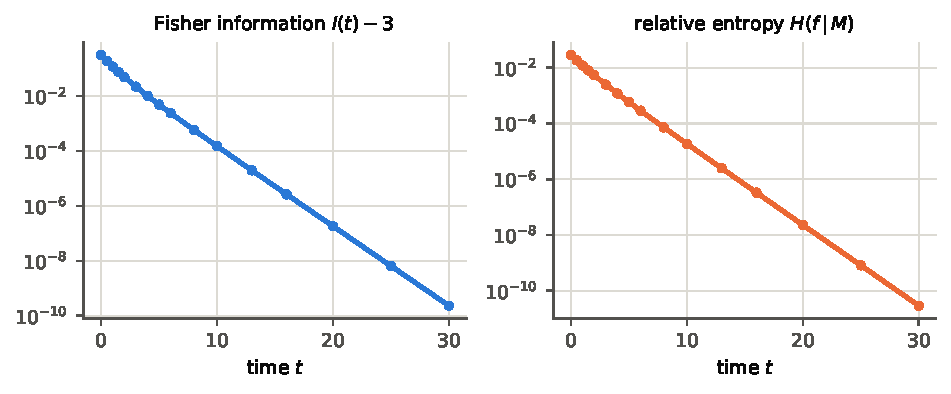
\includegraphics[width=0.92\textwidth]{bkw_fisher_entropy.pdf}
\caption{Fisher information minus its Maxwellian value, and relative entropy, along the exact BKW
solution with $K_0=0.65$. Both decrease monotonically.}
\label{fig:bkw}
\end{figure}

The scope of this check matters. It is an exact special case of the phenomenon Villani's notes
study. It is \emph{not} a test of Theorem~22.6, which is designed for far more singular kernels,
and it makes no claim about the project's retracted \code{gamma\_bound} formula.

\begin{runit}
\begin{verbatim}
python3 verification/validate_fisher_information_monotonicity.py
\end{verbatim}
\end{runit}

\section*{Exercises}
\begin{exercise}\label{ex:bkwpos}
Show that the bracket in Eq.~\eqref{eq:bkw} is positive for all $v$ if and only if $K\ge3/5$
(for $K\le1$).
\end{exercise}
\begin{exercise}\label{ex:fisherM}
Compute $I(M)$ for the unit-temperature Maxwellian in $d$ dimensions, and check the value $3$ used
above for $d=3$.
\end{exercise}
\begin{exercise}\label{ex:bkwtime}
With $K_0=0.65$, how long does it take for $1-K(t)$ to fall below $10^{-3}$?
\end{exercise}

%------------------------------------------------------------------------------------------
\chapter{Villani's Theorem 22.6 and heat-kernel comparison}
\label{ch:villani}
%------------------------------------------------------------------------------------------

\begin{objectives}
\begin{itemize}
  \item state Theorem~22.6 in its literal form and apply it to power-law kernels;
  \item understand the numerical procedure behind its worked examples, and how it was
        independently re-examined;
  \item read the $d=4$ result as what it is: numerical evidence, conditional, offered for checking.
\end{itemize}
\end{objectives}

\section{The statement}

Theorem~22.6 of Villani's lecture notes \cite{villani2025} gives a sufficient condition for the
Fisher information to be nonincreasing along the homogeneous Boltzmann equation. It compares the
angular kernel $\beta$ with a mixture $\beta_0$ of heat kernels on the sphere $S^{d-1}$,
\[
  m\;\le\;\frac{\beta}{\beta_0}\;\le\;M,
\]
and in its literal form concludes monotonicity if
\begin{equation}
  \sup_\theta\;\frac rB\,|\partial_rB|\;\le\;2\sqrt{d\,\frac mM}.
  \label{eq:thm226}
\end{equation}
For power laws, $B=|v-v_*|^\gamma b(\cos\theta)$, the left side is $|\gamma|$, and the condition
becomes $|\gamma|\le\bar\gamma=2\sqrt{d\,m/M}$. The closer $\beta$ is to a heat-kernel mixture,
the closer $m/M$ is to 1 and the larger the range of $\gamma$ covered.

\begin{lesson}[Lesson from the retractions: a real theorem, a wrong formula (R8)]
This project once attributed the formula $\gamma_{\text{bound}}=m_r/M_r+3/2$ to ``Theorem 22.6''.
The attribution was checked by fetching the source. The paper and theorem are real, and the
theorem does involve $m_r/M_r$; but its conclusion is the multiplicative, dimension-dependent
bound \eqref{eq:thm226}, not an additive formula with a $3/2$. Neither the formula nor its value
$1.9513$ appears anywhere in the source. The method was renamed \code{kernel\_regularity\_bounds},
and the number is now described as a convention of this project. The two numbers $1.95$ and
$3.458$ (below) are different objects and must never be compared.
\end{lesson}

\section{The comparison kernels}

The comparison kernels are \emph{subordinated heat kernels},
\[
  b_\omega(\theta)=\int_0^\infty\omega(t)\,t^{-1-\nu/2}\,h_t(\theta)\,dt,
\]
where $h_t$ is the heat kernel on $S^{d-1}$ and $\omega$ is a weight. With $\omega\equiv1$ one
obtains the kernel of the fractional Laplacian $(-\Delta)^{\nu/2}$, which has the same grazing
singularity as the collision kernel. The worked examples in the notes use tuned weights of the
form $1\mp a(1-e^{-bt})$, found ``by trial and error'', and were computed by Silvestre with Julia
code \cite{silvestre2024}. The notes describe the procedure as ``not a purely mathematical proof''.

\section{Re-examination, three ways}

The repository re-executes the authors' Julia code at a pinned commit (it carries no licence, so
it is run, never copied), and adds two implementations written from the mathematics, one in Python
and one in Rust (\code{verification/theorem\_22\_6/}). They share no code with the Julia
repository and take a different numerical route:
\begin{itemize}
  \item the collision kernel comes from classical scattering, parametrised by $\beta=p^2/r_0^2$;
        it reproduces Rutherford's cross-section to $10^{-12}$ in $d=2,3,4$;
  \item each spectral time integral is an exact incomplete gamma function;
  \item both kernels are normalised by exact $\theta\to0$ constants.
\end{itemize}
An exact identity anchors the comparison. At $d=2$, $\nu=1$ (two-dimensional Coulomb
scattering), the symmetrised Rutherford kernel $1/\sin^2\theta$ equals the symmetrised kernel of
$(-\Delta)^{1/2}$ on the circle. The two independent computations agree to $6\times10^{-11}$, and
the bound there is exactly $2\cdot2^{3/4}$.

\paragraph{Results (Level 2).} Both quoted claims reproduce. The minimum of the bound over the
tabulated $\nu$ is $4.355$ in $d=3$ (claim $\ge4.3$; authors' code $4.3568$) and $3.364$ in $d=2$
(claim $>3.3$; authors' code $3.3630$). Rust agrees with Python to $2\times10^{-9}$. One detail
differs: the authors' adaptive quadrature underestimates $\Lambda_b$ as $\nu\to2$, where the
integrand tends to $t^{-1}$. At $d=2$, $\nu=1.999$ it gives $3.932$ against the exact $3.997$,
obtained from
\begin{equation}
  \int_0^\infty t^{-1-s}\bigl(e^{-\alpha t}-e^{-\beta t}\bigr)\,dt=\Gamma(-s)\,(\alpha^s-\beta^s).
  \label{eq:gammaint}
\end{equation}
The error is conservative: the tabulated bounds are slightly low.

\paragraph{Denser sampling (E1).} An infimum sampled on a grid can only be overestimated. With 52
values of $\nu$ and up to 400 angles both claims survive, and the eleven-angle grid overestimates
the bound by at most $0.021$. In $d=2$ a dip appears between the tabulated $\nu=1.0$ and $1.25$:
the minimum is $3.3593$ at $\nu\approx1.06$, still above $3.3$ (Figure~\ref{fig:e1}).

\begin{figure}[htbp]
\centering
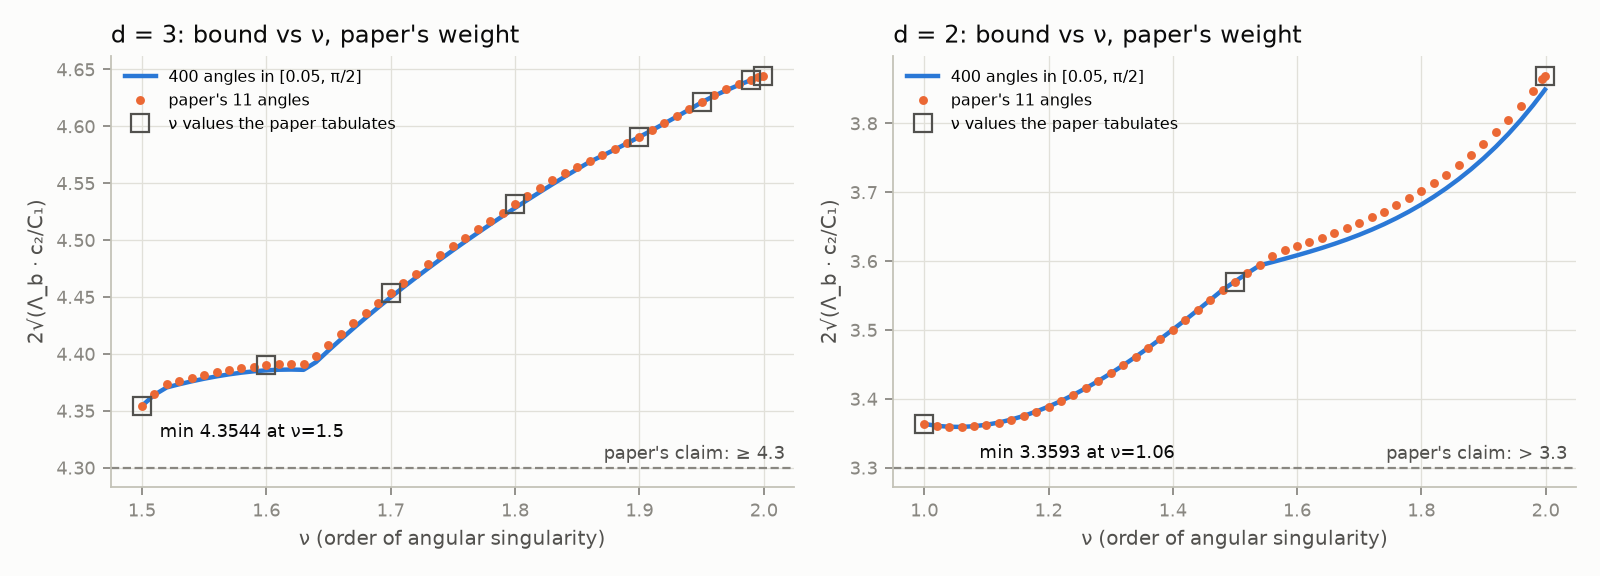
\includegraphics[width=\textwidth]{e1_robustness.png}
\caption{Experiment E1: the bound against $\nu$ with the notes' weights, on 400 angles (line)
and the notes' eleven (dots). Dashed: the claimed thresholds.}
\label{fig:e1}
\end{figure}

\paragraph{The weights (E2).} A grid search over the two-parameter families containing the notes'
weights finds them within $0.06$ of the best in their family. With the plain fractional Laplacian,
both claims fail over most of their range (Figure~\ref{fig:e2}).

\begin{figure}[htbp]
\centering
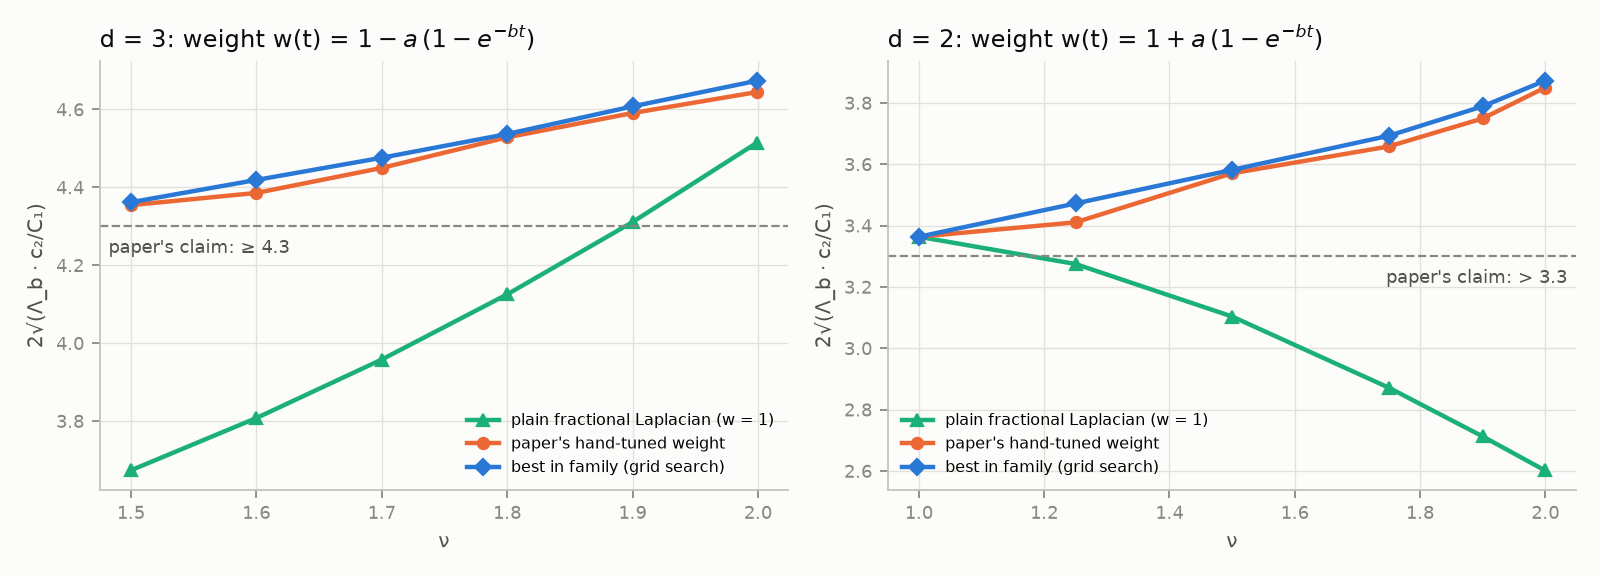
\includegraphics[width=\textwidth]{e2_weight_search.png}
\caption{Experiment E2: plain fractional Laplacian, the notes' weight, and the best weight in its
family.}
\label{fig:e2}
\end{figure}

\section{Applying the theorem to a model kernel (E3)}

The project's phenomenological roton kernel is
$\beta(\cos\theta)=\frac12(1+\cos^2\theta)\,e^{-(1-\cos\theta)/10}$, an analytic model chosen for
its forward-peaked shape, with no measured data in it. After symmetrisation it is close to
$\frac43+\frac23P_2(\cos\theta)$, which a single heat kernel matches at $t=\ln(10)/6\approx0.384$.
A linear program over finite heat-kernel mixtures finds $m/M=0.99654$, with the optimiser landing
at $t=0.3846$ unprompted. In $d=3$ this gives
\[
  \bar\gamma=2\sqrt{3\times0.99654}=3.458,
\]
close to the ceiling $2\sqrt3$ (Figure~\ref{fig:e3}). This is a property of the model kernel, not of
real rotons.

\begin{figure}[htbp]
\centering
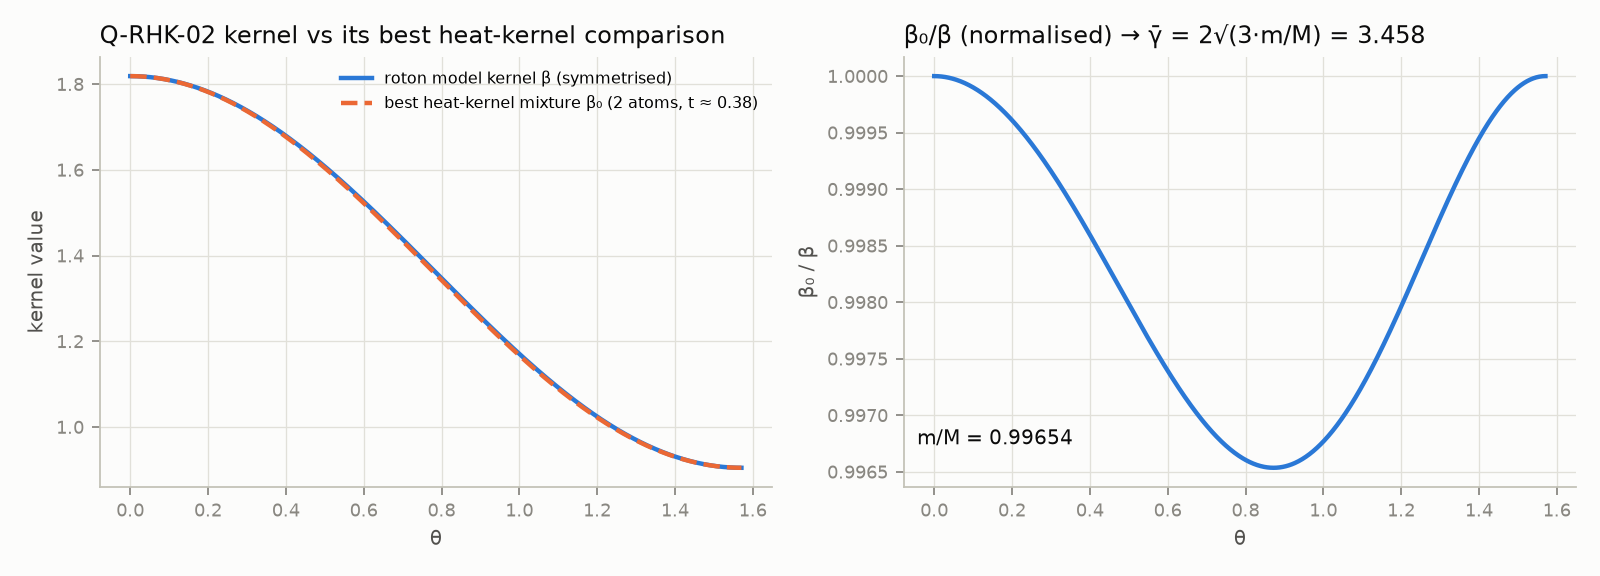
\includegraphics[width=\textwidth]{e3_roton_theorem_22_6.png}
\caption{Experiment E3: the model kernel and its best heat-kernel comparison (left); their ratio,
with $m/M=0.99654$ (right).}
\label{fig:e3}
\end{figure}

\section{The open case in dimension four (E4)}

Remark~22.8 of the notes states that $\gamma\in(-3,-2\sqrt2]$ in $d=4$ is not covered. Classical
scattering by a force $\propto r^{-s}$ in dimension $d$ gives
\[
  \nu=\frac{d-1}{s-1},\qquad\gamma=1-2\nu,
\]
so the open range is $\nu\in[1.9142,2)$, and the literal criterion requires
$m/M>((2\nu-1)/4)^2$, at most $9/16$. A linear program over three admissible families of
comparison kernels (tempered singular kernels with weight $t^{-1-\nu/2}e^{-\mu t}$, bounded
kernels with weight $t^{-1-\nu/2}(1-e^{-bt})$, and pure heat kernels on $S^3$) finds
$m/M\ge0.996$ at sixteen sampled $\nu$, re-checked on 800 angles down to $\theta=0.01$. Hence
$\bar\gamma\approx3.99>|\gamma|$. The result survives halving the basis ($0.9954$) and using the
tempered family alone ($0.9928$). \emph{It fails without tempering}: $m/M$ drops to $0.48$, below
the required $9/16$.

\begin{lesson}[How to read the $d=4$ result]
This is numerical evidence at the standard of the notes' own worked examples, not a proof. It
assumes Theorem~22.6 holds as stated in $d=4$, and below $\theta=0.01$ it relies on the exact
$\theta\to0$ limit. It is offered to the authors for checking. Along the way a numerical artefact
appeared: one spectral cut-off chosen for the smallest angle lost accuracy near $\pi/2$ in $d=4$
and briefly produced $m/M=0.937$. The fix was a per-block cut-off. The general lesson: when a
spectral sum cancels, measure its error against the \emph{smallest} kernel value on the grid.
\end{lesson}

\begin{runit}
\begin{verbatim}
python3 verification/theorem_22_6/reproduce.py                # Python
(cd verification/theorem_22_6/rust && cargo run --release)    # Rust
verification/theorem_22_6/run.sh                              # authors' Julia code
python3 -m pytest tests/test_theorem_22_6_kernels.py -q
\end{verbatim}
The experiments E1--E4b and their run times are listed in
\code{verification/theorem\_22\_6/EXPERIMENTS.md}.
\end{runit}

\section*{Exercises}
\begin{exercise}\label{ex:nurange}
Show that $\gamma\in(-3,-2\sqrt2]$ corresponds to $\nu\in[(1+2\sqrt2)/2,\,2)\approx[1.9142,2)$, and
that the literal criterion in $d=4$ requires $m/M\ge(2\nu-1)^2/16$.
\end{exercise}
\begin{exercise}\label{ex:gammabar}
Compute $\bar\gamma$ in $d=3$ for $m/M=0.99654$, and the ceiling as $m/M\to1$.
\end{exercise}
\begin{exercise}\label{ex:gammaint}
Prove Eq.~\eqref{eq:gammaint} for $0<s<1$ and $\alpha,\beta>0$. Why does naive quadrature struggle
as $s\to1$ in the application above?
\end{exercise}
\begin{exercise}\label{ex:sampling}
Explain why sampling the ratio $\beta/\beta_0$ on a finite set of angles can only
\emph{overestimate} $m/M$, and therefore the bound.
\end{exercise}

%------------------------------------------------------------------------------------------
\chapter{Phase mixing and a second-order response}
\label{ch:phasemixing}
%------------------------------------------------------------------------------------------

\begin{objectives}
\begin{itemize}
  \item compute a second-order Volterra response exactly by Cauchy products;
  \item identify the result with a closed form;
  \item explain phase mixing for free transport, and why a Taylor series at $t=0$ cannot contain a
        plasma echo.
\end{itemize}
\end{objectives}

\section{The protocol}

The protocol QVE-02 takes a linear density response $\rho^{(1)}(t)=\operatorname{sinc}t
=\sin t/t$, forms the field $E^{(1)}=\int_0^t\rho^{(1)}$, the source $S^{(2)}=\rho^{(1)}E^{(1)}$ by
an exact Cauchy product of Taylor series, and one further integration. The engine returns
\begin{equation}
  \rho^{(2)}(t)=\tfrac12t^2-\tfrac1{18}t^4+\tfrac{13}{4050}t^6-\tfrac4{33075}t^8
  +\tfrac{73}{22325625}t^{10}+\mathcal O(t^{12}).
  \label{eq:qve}
\end{equation}
The arithmetic is exact and correct. And $E^{(1)}=\mathrm{Si}(t)$, the sine integral, so
$\rho^{(2)}=\int\rho^{(1)}E^{(1)}=\mathrm{Si}(t)^2/2$. Equation~\eqref{eq:qve} is simply the Taylor
series of $\mathrm{Si}(t)^2/2$, and the test suite now asserts this term by term.

\begin{lesson}[Lesson from the retractions: the echo that was not (R2)]
Earlier versions presented Eq.~\eqref{eq:qve} as the discovery of a nonlinear plasma echo, and a
stored file was labelled ``True 1D1V Vlasov--Poisson phase space simulation'', although no code in
the repository produced it. An echo is a large-time phenomenon: two pulses with distinct
wavenumbers $k_1,k_2$, applied at $0$ and $\tau$, produce a macroscopic response near
$t=\tau k_2/(k_2-k_1)$, long after each linear response has phase-mixed away. A Taylor expansion
about $t=0$ with one input and no phase space cannot contain that. The claim is retracted, and the
protocol is kept as what it is: an exact second-order Volterra response, tested against its
closed form so the identification cannot be lost again.
\end{lesson}

\section{What the input really is}

The positive reading, now proved, concerns the input. Free transport
$\partial_tf+v\,\partial_xf=0$ is solved by $f(x,v,t)=f_0(x-vt,v)$. For a perturbation
$e^{ikx}g(v)$, the density mode is
\[
  \rho_k(t)=\int e^{-ikvt}g(v)\,dv,
\]
the Fourier transform of $g$ at $kt$. For every integrable $g$ it tends to zero
(Riemann--Lebesgue). This is \emph{phase mixing}: nothing is dissipated, but the density
perturbation disappears as the distribution filaments in velocity.

\begin{proposition}[\code{flat\_top\_mode}, \code{flat\_top\_mode\_tendsto\_zero} in
\code{PhaseMixingLink.lean}]
For the flat-top distribution $g=\frac12\mathbb 1_{[-1,1]}$ and $a\ne0$,
$\frac12\int_{-1}^1\cos(av)\,dv=\sin a/a$. Hence the density mode is $\sin(kt)/(kt)$, which
equals QVE-02's input at $k=1$, and $\sin t/t\to0$ as $t\to\infty$, bounded by $1/t$.
\end{proposition}

By Archimedes' hat-box theorem, the one-dimensional marginal of the uniform measure on the sphere
$S^2$ is exactly this flat top, so $\rho^{(1)}$ is also the free-streaming mode of a uniform Fermi
surface; the test suite checks this numerically. The decay is algebraic, like $1/t$, in contrast
with the Gaussian $e^{-k^2t^2/2}$ of a Maxwellian. The second-order term tends to
$\mathrm{Si}(\infty)^2/2=\pi^2/8$: it approaches a constant, and nothing echoes.

\begin{runit}
\begin{verbatim}
python3 -m pytest tests/test_protocols.py -q -k qve_02
python3 -m pytest tests/test_qve02_phase_mixing.py -q
\end{verbatim}
\end{runit}

\section*{Exercises}
\begin{exercise}\label{ex:si}
Using $\mathrm{Si}(t)=t-t^3/18+t^5/600-\cdots$, compute the first three coefficients of
$\mathrm{Si}(t)^2/2$ and compare with Eq.~\eqref{eq:qve}.
\end{exercise}
\begin{exercise}\label{ex:maxwellmode}
Show that the density mode of the unit Maxwellian $g(v)=(2\pi)^{-1/2}e^{-v^2/2}$ is
$e^{-k^2t^2/2}$.
\end{exercise}
\begin{exercise}\label{ex:hatbox}
Show that if a point is uniform on the unit sphere $S^2$, its $z$-coordinate is uniform on
$[-1,1]$ (Archimedes).
\end{exercise}

%==========================================================================================
\part{Practice}
%==========================================================================================

%------------------------------------------------------------------------------------------
\chapter{The engine}
\label{ch:engine}
%------------------------------------------------------------------------------------------

\begin{objectives}
\begin{itemize}
  \item find your way around the repository;
  \item know which stage computes what, and which test protects it;
  \item run the full verification suite.
\end{itemize}
\end{objectives}

\section{Layout}

\begin{center}
\small
\begin{tabular}{>{\ttfamily}l>{\raggedright\arraybackslash}p{9.2cm}}
\toprule
\textrm{Path} & Contents \\
\midrule
agora\_swarm/ & the exact engine: stages and orchestrator \\
tests/ & the pytest suite (49 tests) \\
verification/ & independent numerical checks, data confrontations, Theorem~22.6 experiments \\
simulations/ & protocol drivers and the large-scale simulation \\
lean4\_formalization/ & Lean~4 library \code{AgoraPhysics} \\
alexandrie\_data/ & committed results (small JSON files) \\
notebooks/ & Jupyter notebooks for students \\
agora\_mcp/ & local MCP server (Chapter~\ref{ch:mcp}) \\
docs/ & papers, this book, figures \\
\bottomrule
\end{tabular}
\end{center}

The top-level Markdown files are part of the scientific record: \code{PROTOCOL\_REGISTRY.md}
(what each protocol does), \code{RETRACTIONS.md} (what has been withdrawn),
\code{ROADMAP.md} (what is open), and \code{verification/THEORY\_EXPERIMENT\_LINKS.md} (which
experiment tests which theorem).

\section{Three stages}

The engine is a pipeline. Earlier versions named its stages after living scientists, which
wrongly implied their involvement (R1); they are now named for what they do.
\begin{description}
  \item[\code{LinearResponseStage}] produces exact rational coefficient sequences: the zero-sound
        kernel, the legacy kernel $g$, the linear density perturbation, the model roton kernel.
  \item[\code{KineticStage}] performs the kinetic algebra: \code{pade\_diagonal},
        \code{solve\_zero\_sound\_root}, \code{solve\_zero\_sound\_root\_f0\_f1},
        \code{compute\_second\_order\_volterra\_response} and \code{kernel\_regularity\_bounds}.
  \item[Orchestrator] (\code{agora\_swarm/orchestrator.py}) sequences the protocols, enforces the
        exactness rule at stage boundaries, and writes results as exact strings to the
        \emph{Alexandrie} vault, \code{alexandrie\_data/}.
\end{description}

\section{The protocols}

\begin{center}
\small
\begin{tabular}{l>{\raggedright\arraybackslash}p{5.2cm}>{\raggedright\arraybackslash}p{5.4cm}}
\toprule
ID & What it computes & Status \\
\midrule
QV-01 & zero-sound roots by exact Padé & works at strong coupling; negative result at weak
coupling; extended to $(\Fzs,\Fos)$ \\
QVE-02 & second-order Volterra response & exact; equals $\mathrm{Si}(t)^2/2$; ``echo'' retracted \\
Q-RHK-02 & bounds for a model roton kernel & $1.9513$ is a project convention (R8); Theorem~22.6
gives $\bar\gamma=3.458$ \\
Q-RIP-03 & $L_*=2d$ at $d=2$ & definitional ($2\cdot2=4$), labelled a conjecture (R3) \\
\bottomrule
\end{tabular}
\end{center}

\section{Tests that defend the claims}

Two tests are adversarial by design. One re-derives the kernel from its closed form rather than
comparing it with a table; the other requires float input to raise. Others pin behaviour that
might otherwise be ``fixed'' into a lie: \code{test\_zero\_sound\_weak\_coupling\_has\_no\_admissible\_root}
asserts that the engine keeps reporting \emph{no root} at weak coupling. A test suite that only
checks success cannot protect a negative result; this one does.

\begin{runit}
\begin{verbatim}
python3 -m pytest tests/ -q
python3 verification/validate_zero_sound.py
python3 verification/validate_kernel_regularity_bounds.py
python3 verification/validate_fisher_information_monotonicity.py
python3 verification/theorem_22_6/reproduce.py
python3 verification/helium_kinematics_data.py          # downloads from arXiv
python3 verification/he3_landau/extract_table_ix.py     # downloads from arXiv
python3 verification/he3_landau/zero_sound_real_he3.py
\end{verbatim}
These are the same commands continuous integration runs
(\code{.github/workflows/python\_tests.yml}).
\end{runit}

\section*{Exercises}
\begin{exercise}\label{ex:newtest}
Write a pytest test asserting that \code{solve\_zero\_sound\_root} at $M=1$ returns
$u=15/(9+5F)$ for $F=7/2$, and that it refuses the float \code{3.5}.
\end{exercise}
\begin{exercise}\label{ex:negtest}
Why would a well-meaning contributor be tempted to delete the weak-coupling test, and what would be
lost?
\end{exercise}

%------------------------------------------------------------------------------------------
\chapter{Lean 4 for physicists}
\label{ch:lean}
%------------------------------------------------------------------------------------------

\begin{objectives}
\begin{itemize}
  \item read a short Mathlib proof about real functions;
  \item audit a Lean development with \code{\#print axioms};
  \item state precisely what a Lean theorem certifies in this project.
\end{itemize}
\end{objectives}

\section{Setting up}

The library \code{AgoraPhysics} lives in \code{lean4\_formalization/}. It pins the toolchain
\code{leanprover/lean4:v4.31.0} and Mathlib at revision \code{ec6e08b4}. Always fetch Mathlib's
compiled cache: compiling Mathlib from source takes hours.

\begin{runit}
\begin{verbatim}
cd lean4_formalization
lake exe cache get
lake build
\end{verbatim}
The default target is the library, not the executable: building the executable would force native
compilation of all of Mathlib just to link a binary that prints a greeting.
\end{runit}

\section{Reading a proof: the upper edge}

Here is the upper edge of the zero-sound bracket, verbatim from \code{ZeroSoundBracket.lean}:
\begin{lstlisting}
noncomputable def g3 (s : ℝ) : ℝ := s / 2 * log ((s + 1) / (s - 1)) - 1

theorem root_upper {F s : ℝ} (hF : 0 < F) (hs : 1 < s) (hroot : g3 s = 1 / F) : s - 1 ≤ F := by
  have h1 : 0 < s - 1 := by linarith
  have h := g3_le hs
  rw [hroot] at h
  exact (one_div_le_one_div hF h1).mp h
\end{lstlisting}
Read it as a physicist would.
\begin{enumerate}
  \item \code{g3} is $\chi(s)$ as a function of $s$, over the real numbers.
  \item The hypotheses are $F>0$, $s>1$ (undamped) and that $s$ is a root.
  \item \code{g3\_le} is the lemma $g_3(s)\le1/(s-1)$, from $\ln y\le y-1$.
  \item Rewriting with the root equation turns it into $1/F\le1/(s-1)$.
  \item Since both sides are positive, inverting reverses the inequality: $s-1\le F$.
\end{enumerate}
Each tactic is a small, checkable step: \code{linarith} solves linear arithmetic, \code{rw}
rewrites with an equation, and \code{one\_div\_le\_one\_div} is a Mathlib lemma.

The lower edge, \code{root\_lower}, follows the same pattern with the bound
$g_3(s)\ge\frac12\ln\frac2{s-1}-1$ and then exponentiates. Its docstring notes that it does not
need $F>0$: \code{g3\_pos} rules out a root for $F<0$, and in Lean $1/0=0$ rules it out for $F=0$.
Details like this are what a proof assistant forces you to face.

\section{A proof about phase mixing}

\begin{lstlisting}
theorem flat_top_mode_tendsto_zero : Tendsto (fun t : ℝ => sin t / t) atTop (𝓝 0) := by
  have hinv : Tendsto (fun t : ℝ => t⁻¹) atTop (𝓝 0) := tendsto_inv_atTop_zero
  have hbound : ∀ᶠ t : ℝ in atTop, ‖sin t / t‖ ≤ t⁻¹ := by
    filter_upwards [eventually_gt_atTop 0] with t ht
    rw [Real.norm_eq_abs, abs_div, abs_of_pos ht, div_eq_mul_inv]
    exact mul_le_of_le_one_left (inv_nonneg.mpr ht.le) (abs_sin_le_one t)
  exact squeeze_zero_norm' hbound hinv
\end{lstlisting}
The structure is the textbook squeeze argument: $1/t\to0$, and $|\sin t/t|\le1/t$ eventually, so
$\sin t/t\to0$. \code{Tendsto \dots\ atTop} $(\mathcal{N}\,0)$ is Mathlib's way of writing
$\lim_{t\to\infty}=0$ with filters.

\section{The axiom audit}

Every Lean file of the project ends with lines such as
\begin{lstlisting}
#print axioms AgoraPhysics.ZeroSoundBracket.zero_sound_bracket
\end{lstlisting}
The build log then lists the axioms each theorem depends on. Only the three standard axioms of
Mathlib are acceptable: \code{propext}, \code{Classical.choice} and \code{Quot.sound}. If
\code{sorryAx} appears, a proof is incomplete somewhere upstream, even if the file itself contains
no \code{sorry}. Continuous integration fails in that case.

\begin{lesson}[Lesson from the development: a proof that silently was not]
While writing \code{PhaseMixingLink.lean}, a \code{simpa} step failed to close its goal in the
expected shape. Lean elaborated the theorem with \code{sorryAx} standing in for the failed step,
and it was the axiom audit that flagged it. Restating the bound in norm form fixed it. A green build is not a proof;
an axiom list is evidence.
\end{lesson}

\section{What the Lean library certifies}

\begin{itemize}
  \item \code{Protocols.lean}: arithmetic identities, such as the $[1/1]$ order condition
        $a_2+q_1a_1=0$ and the fact that $u=10/37$ is a root of $Q-\frac{93}{10}P$. Two theorems
        there are labelled vacuous in the source itself: one proves $2\cdot2=4$ after unfolding a
        definition, one has its hypothesis as its conclusion (R3). They are kept, labelled, as a
        record.
  \item \code{ZeroSoundBracket.lean}: real analysis about the Landau zero-sound relation
        (Theorem~\ref{thm:bracket}).
  \item \code{PhaseMixingLink.lean}: real analysis about free transport.
\end{itemize}
None of these certifies anything about real $^3$He or $^4$He. That connection, where it is made,
is made by the data comparisons of Chapter~\ref{ch:data}. Lemmas \code{g3\_pos}, \code{g3\_le}
and \code{g3\_ge} are restated, with attribution, from a companion project,
SocrateAI-Scientific-QuantumFluids, which pins a different Lean version.

\section*{Exercises}
\begin{exercise}\label{ex:hF}
Explain in words why \code{root\_lower} needs no hypothesis $F>0$, including the case $F=0$.
\end{exercise}
\begin{exercise}\label{ex:vacuous}
The theorem \code{admissible\_singularity\_limit (h : $\gamma$ < gamma\_bound) : $\gamma$ < 16063/8232}
with \code{gamma\_bound := 16063/8232} is proved by \code{exact h}. What does it establish?
\end{exercise}

%------------------------------------------------------------------------------------------
\chapter{Confronting models with data}
\label{ch:data}
%------------------------------------------------------------------------------------------

\begin{objectives}
\begin{itemize}
  \item derive Landau parameters of real $^3$He from published thermodynamic tables;
  \item see a mathematically correct model fail on real parameters, and repair it;
  \item test machine-checked kinematic statements on open neutron-scattering data for $^4$He.
\end{itemize}
\end{objectives}

\section{Getting data honestly}

Two rules govern data in this project. Every value is fetched from a named source by code, with a
checksum where possible, and never typed from memory. And third-party files are not redistributed:
the scripts download them to a cache.

\begin{lesson}[Lesson from the retractions: ``no dataset exists'' (R9)]
After a search of Zenodo, Hugging Face, Materials Cloud and the ILL portal, the project once
concluded that no open data existed for the roton regime of $^4$He. That was wrong: the authors
of Godfrin \emph{et al.}\ 2021 \cite{godfrin2021} had published their dispersion data as arXiv
\emph{ancillary files}, and the search had not looked there. A negative search result is a claim
about the search, not about the world.
\end{lesson}

\section{Real \texorpdfstring{$^3$He}{3He}: Landau parameters from thermodynamics}

Kollar and Vollhardt \cite{kollar2000} tabulate, from Greywall's measurements \cite{greywall1983},
the molar volume $V$, the specific-heat coefficient $\gamma/R$ and the compressibility $\kappa$
of normal liquid $^3$He at $T\to0$, from 0 to 29~bar (their Table~IX). The script
\code{extract\_table\_ix.py} fetches their arXiv PDF, reads page~19 from its \emph{text layer}
(no OCR), keeps each value exactly as printed, and checks the table internally:
\begin{itemize}
  \item the $\partial\gamma/\partial P$ column against finite differences of $\gamma$, to
        $2.4\times10^{-3}$;
  \item $\kappa$ against $-V^{-1}\partial V/\partial P$, to $6.8\times10^{-3}$;
  \item the prefactor of their Eq.~(30) recomputed from CODATA constants, $3.2869\times10^{-4}$
        against the printed $3.285\times10^{-4}$.
\end{itemize}
From $\gamma$ follows the effective mass, $m^*/m=(2/\pi^2)(\gamma/R)\,T_F$, with $T_F$ the bare
Fermi temperature at that density; then $\Fos=3(m^*/m-1)$. From $\kappa$ and their Eq.~(30)
follows $\Fzs$. At 0~bar: $V=36.846$~cm$^3$, $\gamma/R=2.7411$, $T_F=4.957$~K, $m^*/m=2.753$,
$\Fos=5.260$, $\Fzs=10.28$, $v_F=60.04$~m/s.

\section{The one-parameter model fails}

Table~\ref{tab:he3} and Figure~\ref{fig:he3} show the outcome (Level~4). With $\Fzs$ alone, the
model predicts zero sound \emph{slower} than first sound at every pressure. In $^3$He zero sound
is slightly faster. The model is exact as mathematics and wrong as physics, and only real
parameters could show it. Adding $\Fos$ restores the observed ordering, with $c_0/c_1=1.036$ at
0~bar falling to $1.005$ at 29~bar. First sound computed from Landau theory, Eq.~\eqref{eq:c1},
agrees with the thermodynamic $1/\sqrt{\rho\kappa}$ from the same table to $2\times10^{-10}$, and
the exact $[4/4]$ root of Eq.~\eqref{eq:f0f1poly} agrees with a 60-digit reference to better than
$10^{-8}$ at 0 and 29~bar.

\begin{table}[htbp]
\centering
\caption{Zero sound $c_0$ and first sound $c_1$ (m/s) in liquid $^3$He from the Landau parameters
of \cite{kollar2000} (\code{alexandrie\_data/HE3-LANDAU/zero\_sound\_real\_he3.json}).}
\label{tab:he3}
\begin{tabular}{rrrrrrr}
\toprule
$P$ (bar) & $\Fzs$ & $\Fos$ & $c_0$, $\Fzs$ only & $c_0$, $(\Fzs,\Fos)$ & $c_1$ & $c_0/c_1$ \\
\midrule
0  & 10.28 & 5.26  & 120.8 & 200.1 & 193.2 & 1.036 \\
6  & 21.43 & 7.29  & 140.5 & 260.1 & 255.5 & 1.018 \\
15 & 41.95 & 9.69  & 161.9 & 332.9 & 329.9 & 1.009 \\
29 & 73.94 & 13.00 & 174.4 & 402.7 & 400.6 & 1.005 \\
\bottomrule
\end{tabular}
\end{table}

\begin{figure}[htbp]
\centering
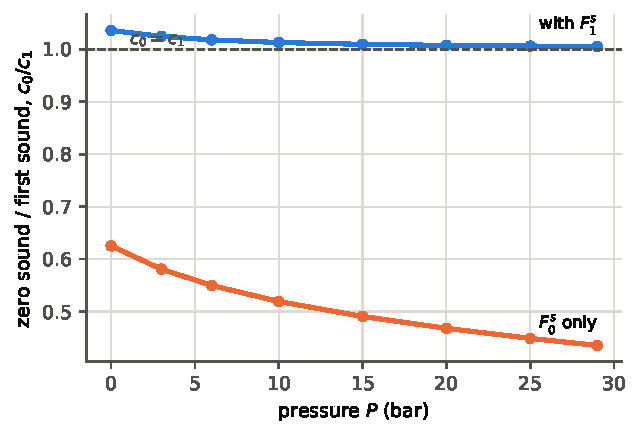
\includegraphics[width=0.72\textwidth]{he3_c0_over_c1.pdf}
\caption{Ratio of zero sound to first sound for real $^3$He, all eight computed pressures. With
$\Fzs$ alone the ratio is below one, which is wrong.}
\label{fig:he3}
\end{figure}

One caveat: the absolute $c_1=193$~m/s at 0~bar is about $5\%$ above commonly quoted
measurements, and the source notes that its compressibility is least certain below about 2~bar.
Ratios are more reliable here than absolute speeds. The model also neglects $F_2^s$ and higher,
finite temperature and collisions.

\section{Real \texorpdfstring{$^4$He}{4He}: neutron data and machine-checked kinematics}

Superfluid $^4$He has a single excitation branch $\varepsilon(Q)$: phonons at small $Q$, a local
maximum (the \emph{maxon}) and a local minimum (the \emph{roton}, with gap $\Delta$). A companion
project formalises kinematic statements about such a branch. The script
\code{helium\_kinematics\_data.py} tests them on the IN5 dispersion data of \cite{godfrin2021}:
seven pressures from 0 to 24.08~bar, with per-point uncertainties. The files are fetched from arXiv
and checked by SHA-256. The fit reproduces the published sound velocity ($1.5685$ against
$1.5679$~meV\,\AA) and roton gap ($0.7417$ against $0.7445$~meV).

\paragraph{Maxon versus the roton-pair threshold.} A maxon above $2\Delta$ can decay into two
rotons. The data show the maxon below $2\Delta$ up to 10~bar and above it at 24.08~bar,
by $+0.0106\pm0.0005$~meV, about $21\sigma$ (Figure~\ref{fig:he4}), as Beauvois \emph{et al.}\
reported \cite{beauvois2018}. A proved lemma adds something the data alone cannot: whether an
energy exceeds $2\Delta$ cannot be changed by a proportional recalibration of the energy scale, so
no such calibration error can reverse the conclusion.

\begin{figure}[htbp]
\centering
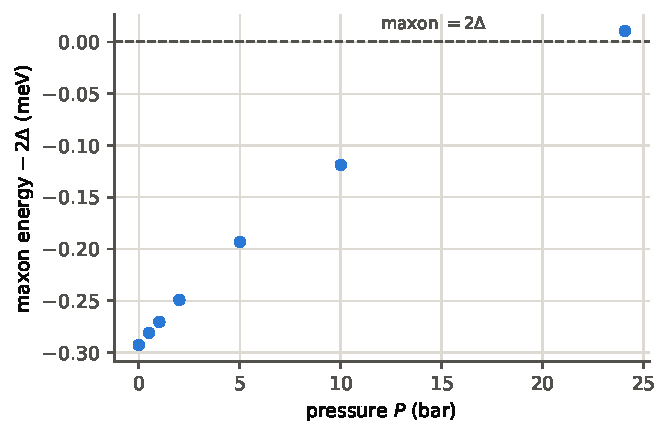
\includegraphics[width=0.72\textwidth]{he4_maxon_minus_2delta.pdf}
\caption{Maxon energy minus twice the roton gap, from the IN5 dispersion of \cite{godfrin2021}
(\code{alexandrie\_data/HE4-KIN/helium\_kinematics.json}). Error bars are one standard
deviation.}
\label{fig:he4}
\end{figure}

\paragraph{Three-phonon decay.} For $\varepsilon=cQ(1+aQ^2)$, a proved equivalence says that
three-phonon decay is open if and only if $a\ge0$. At saturated vapour pressure a fit on
$Q\le0.15$~\AA$^{-1}$ gives $a=+0.95\pm0.25$~\AA$^2$, upward curvature at $3.8\sigma$, so decay is
open. The sign change reported near 18--20~bar cannot be decided from these files, which start
at $Q=0.15$~\AA$^{-1}$ for $P>0$.

\begin{lesson}[Lesson from the development: a test that asked too much]
The first version of this test asserted the 18--20~bar sign change, which the data cannot
resolve, and required $2\sigma$ significance on every fit range. It was redesigned to report
``undecided'' where the data are silent and to treat a non-significant result as ``not
contradicted'' rather than as a failure. The change is recorded in the repository, not hidden.
\end{lesson}

\begin{runit}
\begin{verbatim}
python3 verification/he3_landau/extract_table_ix.py
python3 verification/he3_landau/zero_sound_real_he3.py
python3 verification/helium_kinematics_data.py
\end{verbatim}
\end{runit}

\section*{Exercises}
\begin{exercise}\label{ex:mstar}
From $\gamma/R=2.7411$ and $T_F=4.9569$~K at 0~bar, compute $m^*/m$ and $\Fos$.
\end{exercise}
\begin{exercise}\label{ex:c1}
With $v_F=60.042$~m/s, $\Fzs=10.2788$ and $\Fos=5.2601$, compute $c_1$ from Eq.~\eqref{eq:c1}.
\end{exercise}
\begin{exercise}\label{ex:recal}
Prove the recalibration lemma: if every energy is multiplied by the same $\lambda>0$, the sign of
$\varepsilon_{\text{maxon}}-2\Delta$ is unchanged.
\end{exercise}
\begin{exercise}\label{ex:sigma}
The excess at 24.08~bar is $0.0106\pm0.0005$~meV. How many standard deviations is that, and what
assumption does ``$21\sigma$'' rely on?
\end{exercise}

%------------------------------------------------------------------------------------------
\chapter{A large simulation certified by an exact solution}
\label{ch:simulation}
%------------------------------------------------------------------------------------------

\begin{objectives}
\begin{itemize}
  \item simulate the homogeneous Boltzmann equation with a stochastic particle method (DSMC);
  \item judge a floating-point simulation against an exact solution, with no fitted parameter;
  \item recognise the Monte Carlo error law $N^{-1/2}$ and a discretisation bias.
\end{itemize}
\end{objectives}

\section{The idea}

The project's rule is that an exact result certifies a floating-point computation, never the
reverse. The large simulation applies that rule at scale. The floating-point computation is a
Direct Simulation Monte Carlo (DSMC) method of Nanbu--Bird type with up to $10^6$ particles; the
exact result is the BKW solution of Chapter~\ref{ch:kinetic}. The simulation is judged against the
exact curves, and its error must shrink like $N^{-1/2}$. Nothing is fitted.

\section{The model}

The script \code{simulations/large\_scale/dsmc\_bkw.py} treats 3D Maxwell molecules with
isotropic scattering, normalised so that every particle collides at rate one:
\[
  \partial_tf=Q^+(f,f)-f,\qquad
  Q^+(f,f)(v)=\iint f(v')f(v_*')\,dv_*\,\frac{d\omega}{4\pi}.
\]
A collision of $v$ and $w$ keeps the centre of mass $V=(v+w)/2$ and the relative speed
$|u|=|v-w|$, and sends
\[
  v'=V+\tfrac12|u|\,\omega,\qquad w'=V-\tfrac12|u|\,\omega,\qquad\omega\text{ uniform on }S^2.
\]

\section{The exact benchmark}

Averaging one collision over $\omega$ and over independent, isotropic partners gives a closed
equation for the fourth moment $m_4=\mathbb E|v|^4$:
\begin{equation}
  \frac{dm_4}{dt}=-\frac13\left(m_4-\frac53m_2^2\right),
\end{equation}
so $m_4$ relaxes at rate exactly $1/3$ toward $15$ when $m_2=3$. For BKW,
$m_4-15=-15(1-K)^2$ (Chapter~\ref{ch:kinetic}), and the moment equation forces
$(1-K)^2\propto e^{-t/3}$, that is $K(t)=1-(1-K_0)e^{-t/6}$. The time scale is \emph{derived}
for this normalisation, not fitted. The script also uses $m_6=315K^2-210K^3$, the exact marginal
distribution of $v_x$, and the relative entropy computed by quadrature.

\section{The algorithm}

Collisions form a Poisson process with total rate $N/2$. Each step of length $\Delta t$ draws
$k\sim\mathrm{Poisson}(N\Delta t/2)$ and collides $k$ disjoint random pairs. The only
approximation is disjointness within a step: the per-step contraction of $m_4-15$ becomes
$1-\Delta t/3$ instead of $e^{-\Delta t/3}$. The script computes the effect of this on $m_4$ in
closed form and reports it. In the committed run, with $\Delta t=10^{-2}$, it is at most
$1.0\times10^{-4}$ relative on $m_4$, below the Monte Carlo error even at $N=10^6$. The cost is proportional to the number of collisions, $\mathcal O(NT)$, independent of
$\Delta t$.

The default initial condition is $K_0=3/5$, the extreme member of the BKW family, where $f$
vanishes at $v=0$. The initial particles are sampled from that exact $f$.

\section{What to look for}

\begin{itemize}
  \item \textbf{Moments.} $m_4(t)$ and $m_6(t)$ from particles should follow the exact curves
        within statistical error bars.
  \item \textbf{Error law.} Repeating with $N=10^4,10^5,10^6$ and several seeds, the error should
        fall like $N^{-1/2}$: a factor of about $3.2$ per decade of $N$. A slower decay would
        reveal a bias, for example from the time step.
  \item \textbf{Entropy.} The relative entropy is estimated from a histogram of speeds. Its exact
        counterpart is the same binned divergence of the exact $f$; binning only lowers it
        (data-processing inequality). Both must decrease.
\end{itemize}
\section{Results}

The committed summary \code{alexandrie\_data/SIMULATIONS/dsmc\_bkw\_summary.json} records the
maintainers' run to $t=30$ from $K_0=3/5$ (Table~\ref{tab:dsmc}). The root-mean-square relative
error of $m_4$ over the trajectory falls from $6.8\times10^{-3}$ at $N=10^4$ to $6.2\times10^{-4}$
at $N=10^6$, and a fit of $\log(\text{error})$ against $\log N$ gives slope $-0.519$, against the
Monte Carlo prediction $-1/2$. Energy is conserved to rounding ($\sim10^{-15}$). The exact relative
entropy decreases strictly, from $0.0639$ to $4.9\times10^{-11}$, and the particle estimate
follows it with an error that also shrinks with $N$. Nothing was fitted: the only inputs are the
collision rule and the initial $f$. The numbers were current when this book was written; the
notebook regenerates them. Large raw output is written to a cache directory, not to git.

\begin{table}[htbp]
\centering
\caption{DSMC against the exact BKW solution: root-mean-square errors over $0\le t\le30$, averaged
over seeds (\code{dsmc\_bkw\_summary.json}).}
\label{tab:dsmc}
\begin{tabular}{rrrrrr}
\toprule
$N$ & seeds & rel.\ error $m_4$ & rel.\ error $m_6$ & abs.\ error $H$ & wall time (s) \\
\midrule
$10^4$ & 16 & $6.8\times10^{-3}$ & $2.2\times10^{-2}$ & $2.1\times10^{-3}$ & 5 \\
$10^5$ & 4  & $2.0\times10^{-3}$ & $6.4\times10^{-3}$ & $3.1\times10^{-4}$ & 17 \\
$10^6$ & 2  & $6.2\times10^{-4}$ & $2.1\times10^{-3}$ & $4.8\times10^{-5}$ & 135 \\
\bottomrule
\end{tabular}
\end{table}

\begin{runit}
\begin{verbatim}
python3 simulations/large_scale/dsmc_bkw.py --quick     # < 30 s, as in CI
python3 simulations/large_scale/dsmc_bkw.py             # N = 1e4, 1e5, 1e6, a few minutes
python3 simulations/large_scale/he3_pressure_sweep.py   # exact solver over all pressures
jupyter notebook notebooks/04_large_simulation_dsmc_vs_exact_bkw.ipynb
\end{verbatim}
The notebooks \code{01\_exact\_zero\_sound\_quickstart}, \code{02\_real\_he3\_zero\_sound} and
\code{03\_theorem\_22\_6\_numerics} accompany Chapters~\ref{ch:zerosound}, \ref{ch:data} and
\ref{ch:villani}.
\end{runit}

\section*{Exercises}
\begin{exercise}\label{ex:m4}
Check that $m_4=30K-15K^2$ satisfies the moment equation when $K(t)=1-(1-K_0)e^{-t/6}$.
\end{exercise}
\begin{exercise}\label{ex:mcerr}
With $N=10^6$ particles, estimate the standard error of the particle average of $|v|^4$ at
equilibrium, given that $\mathrm{Var}(|v|^4)=\mathbb E|v|^8-15^2$ and $\mathbb E|v|^8=945$ for the
unit Maxwellian.
\end{exercise}
\begin{exercise}\label{ex:bias}
Over a time $T$ with step $\Delta t$, compare $(1-\Delta t/3)^{T/\Delta t}$ with $e^{-T/3}$ for
$T=30$, $\Delta t=10^{-2}$. Why can this bias be computed exactly rather than estimated?
\end{exercise}

%------------------------------------------------------------------------------------------
\chapter{The MCP server: the engine as a tool for AI agents}
\label{ch:mcp}
%------------------------------------------------------------------------------------------

\begin{objectives}
\begin{itemize}
  \item start the local MCP server and connect a client to it;
  \item know what each tool computes and what it refuses.
\end{itemize}
\end{objectives}

The Model Context Protocol (MCP) lets an AI assistant call tools provided by a local program. The
package \code{agora\_mcp} exposes the engine as such a server, over standard input and output, on
the same machine. It is started with
\begin{verbatim}
python3 -m agora_mcp
\end{verbatim}
and the repository's \code{.mcp.json} registers it for Claude Code as \code{agora-physics}. Full
documentation is in \code{docs/MCP.md}.

\begin{center}
\small
\begin{tabular}{>{\ttfamily}l>{\raggedright\arraybackslash}p{9.6cm}}
\toprule
\textrm{Tool} & What it does \\
\midrule
zero\_sound\_root & exact Padé root for $(\Fzs,\Fos)$ at order $M$ \\
pade\_approximant & exact $[M/M]$ approximant of the zero-sound kernel \\
he3\_landau\_parameters & real $^3$He parameters at a tabulated pressure, with provenance \\
helium\_kinematics & committed results of the $^4$He data tests \\
theorem\_22\_6\_bound & kernel comparison behind Theorem~22.6's worked examples \\
list\_protocols & the protocols and the whitelisted verification scripts \\
get\_retractions & the entries of \code{RETRACTIONS.md} \\
run\_verification & runs one whitelisted verification script \\
\bottomrule
\end{tabular}
\end{center}

The server applies the same rules as the engine. Numbers are sent as strings or fractions
(\code{"93/10"}); a JSON float is refused with an explanation, for the reason of
Chapter~\ref{ch:exact}. The data tools serve only tabulated values, without interpolation, and
return their source. \code{run\_verification} runs only whitelisted scripts, and scripts that
download data run only if the server was started with \code{AGORA\_MCP\_ALLOW\_NETWORK=1}.

\begin{runit}
In Claude Code, from the repository root, the server is picked up from \code{.mcp.json}. Then
ask, for example: ``Use \code{zero\_sound\_root} with F0s = 10.279 and F1s = 5.260 at M = 4, and
compare with the first sound in \code{he3\_landau\_parameters} at 0 bar.''
\end{runit}

\section*{Exercises}
\begin{exercise}\label{ex:mcpfloat}
Why does the server refuse the JSON number \code{9.3} but accept the string \code{"9.3"}? What
exact value does the string become?
\end{exercise}

%------------------------------------------------------------------------------------------
\chapter{Contributing as a scientist or an AI agent}
\label{ch:contrib}
%------------------------------------------------------------------------------------------

\begin{objectives}
\begin{itemize}
  \item choose the right channel for a contribution;
  \item write a numeric-calculation request that an agent can execute;
  \item prepare a pull request that meets the project's standard.
\end{itemize}
\end{objectives}

\section{Channels}

The repository's \code{CONTRIBUTING.md} describes the process and \code{AGENTS.md} the rules. In
brief, there are four kinds of contribution.
\begin{enumerate}
  \item \textbf{Numeric calculation request.} Open an issue with the form of that name. Give exact
        inputs (as rationals where possible), the quantity wanted, the precision or evidence level
        needed, and the source of any physical input. Fully specified requests are labelled
        \code{agent-ready}.
  \item \textbf{Roadmap proposal.} Propose a protocol, a dataset to confront, a theorem to
        formalise or a method to replace. State what would count as success \emph{and} what would
        count as a negative result.
  \item \textbf{Scientific error or retraction.} If a claim is wrong, overstated or mis-attributed,
        report it. This is the most valuable contribution. Confirmed errors enter
        \code{RETRACTIONS.md} with credit, and are fixed everywhere the claim appears.
  \item \textbf{Code, proofs, data, documents} through pull requests.
\end{enumerate}

\section{Rules for everyone, human or agent}

The rules in \code{AGENTS.md} are the ones this book has motivated chapter by chapter:
\begin{itemize}
  \item no floats in derivations (Chapter~\ref{ch:exact});
  \item no numbers from memory: fetch from a named source, in code (Chapter~\ref{ch:data});
  \item label every claim with its evidence level, and never call numerical evidence a proof;
  \item read \code{RETRACTIONS.md} first, never re-introduce a retracted claim, and when a claim is
        withdrawn, search the \emph{whole} repository for it;
  \item Lean proofs audited with \code{\#print axioms}, not grep (Chapter~\ref{ch:lean});
  \item negative results are results, and are tested (Chapter~\ref{ch:zerosound});
  \item no person-named agents, no implied endorsement, no copying of unlicensed code;
  \item no secrets in code, logs or commits; big data stays out of git.
\end{itemize}

\begin{lesson}[Lesson from the history: fixes that stopped at one file]
Several retractions were first fixed in one place but not in others that repeated the claim: the
``echo'' framing survived in the orchestrator's printed output and in a Lean theorem name after it
had been removed from the Python stage. When a claim is withdrawn, grep the code, the
orchestrator, the persisted JSON, the Lean names and comments, and the LaTeX.
\end{lesson}

\section{AI agents}

Agents are first-class contributors under the same rules. Claude Code reads the repository's
\code{CLAUDE.md}, which imports \code{AGENTS.md}, and can use the local MCP server. Google Jules
reads \code{AGENTS.md} and works in its own virtual machine, using the scripts and tests directly.
Agent pull requests say that they are agent-authored and name the tool; a human maintainer merges.

\section{A worked request}

\begin{example}[From question to merged result]
\label{ex:request}
A student asks: ``What is the zero-sound velocity at 15~bar with $\Fzs$ and $\Fos$, at Padé order
6, and how far is it from the $[4/4]$ value?'' A good issue states the inputs with their source
(\code{he3\_landau\_parameters} at 15~bar, from \cite{kollar2000}), the quantity (the root of
Eq.~\eqref{eq:f0f1poly} at $M=6$ and $M=4$, and their relative difference), and the evidence level
(Level~1 for the roots, Level~2 for a 60-digit comparison). An agent then adds a test or script,
commits a small JSON result under \code{alexandrie\_data/}, and opens a pull request whose
description quotes the numbers and their level. Continuous integration re-runs everything.
\end{example}

\section*{Exercises}
\begin{exercise}\label{ex:badrequest}
Rewrite this request so that an agent can execute it: ``Can you check whether zero sound works
for helium at high pressure?''
\end{exercise}

\appendix

%------------------------------------------------------------------------------------------
\chapter{Solutions to the exercises}
\label{app:solutions}
%------------------------------------------------------------------------------------------

\paragraph{\ref{ex:float-roundtrip}.} \code{float(1/1001)} is close to $0.000999001$, and the best
rational approximation with denominator at most 1000 is $1/1000$. The parameter has been
silently replaced by a different one, with a relative change of $10^{-3}$. Worse than the size of
the change is that nothing reports it: every later exact computation is exact for the wrong
input.

\paragraph{\ref{ex:levels}.} (a) Level~1. (b) Level~2. (c) Level~3 (Theorem~\ref{thm:bracket}).
(d) Level~4: it is a statement about measurement; the project's model reproduces it only with
$\Fos$. (e) No evidence: it was retracted (R3).

\paragraph{\ref{ex:tabletest}.} A table test checks that code and table agree. If both came from
the same wrong source, or the table was invented and the code made to match it, the test passes. A
closed-form test compares against an independent derivation, so a wrong table fails.

\paragraph{\ref{ex:padeexp}.} With $a_0=1,a_1=1,a_2=1/2$: $a_2+q_1a_1=0$ gives $q_1=-1/2$, then
$p_0=1$, $p_1=a_1+q_1a_0=1/2$. So $e^x\approx(1+x/2)/(1-x/2)$, which is $3$ at $x=1$, against
$e=2.71828$ and the Taylor value $2.5$. Both use three coefficients; here the Taylor polynomial is
slightly closer, but the Padé form keeps the symmetry $R(-x)=1/R(x)$ of the exponential.

\paragraph{\ref{ex:pade22}.} The conditions for $n=3,4$ are
$a_3+q_1a_2+q_2a_1=0$ and $a_4+q_1a_3+q_2a_2=0$, i.e.
$\frac17+\frac{q_1}5+\frac{q_2}3=0$ and $\frac19+\frac{q_1}7+\frac{q_2}5=0$. Their solution is
$q_1=-10/9$, $q_2=5/21$. Then $p_0=0$, $p_1=a_1=1/3$, $p_2=a_2+q_1a_1=\frac15-\frac{10}{27}
=-\frac{23}{135}$.

\paragraph{\ref{ex:singular}.} For $A=1+u^2$ (so $a_1=0$, $a_2=1$), the $[1/1]$ condition
$a_2+q_1a_1=0$ reads $1=0$: no solution. An exact engine must report that the approximant does not
exist. A least-squares fallback would return \emph{some} rational function that satisfies no order
condition, and every root computed from it would look exact while meaning nothing.

\paragraph{\ref{ex:ak}.} $\frac s2\ln\frac{s+1}{s-1}=s\operatorname{artanh}(1/s)
=\sum_{k\ge0}\frac{s^{-2k}}{2k+1}=1+\sum_{k\ge1}\frac{u^k}{2k+1}$. Subtracting 1 gives
$a_k=1/(2k+1)$: $1/3,1/5,1/7$.

\paragraph{\ref{ex:root11}.} $Q-FP=1-\frac{3u}5-\frac{Fu}3=0$ gives $u=\frac{1}{3/5+F/3}
=\frac{15}{9+5F}$. Then $u<1$ iff $15<9+5F$ iff $F>6/5$; and $u>0$ for $F>0$.

\paragraph{\ref{ex:bracket93}.} Lower edge: $2e^{-(2+2/9.3)}=0.2183$. Upper edge: $9.3$. The $M=1$
value gives $s-1=0.9235$, inside. The upper edge comes from $\ln y\le y-1$, which is tight only
for $y$ near $1$, i.e.\ for $s$ large; at strong coupling the root is at moderate $s$, where the
inequality is far from equality.

\paragraph{\ref{ex:f1zero}.} With $\Fos=0$, $a=1$ and the polynomial is
$P\,\Fzs u-Qu=u(\Fzs P-Q)$. The extra root is $u=0$, i.e.\ $s=\infty$, which is excluded because
admissible roots must lie in the open interval $(0,1)$.

\paragraph{\ref{ex:bkwpos}.} The bracket is $\frac{5K-3}{2K}+\frac{1-K}{2K^2}|v|^2$. For $K\le1$
the second coefficient is nonnegative, so the minimum is at $v=0$, where the value is
$(5K-3)/(2K)$. It is nonnegative iff $K\ge3/5$.

\paragraph{\ref{ex:fisherM}.} $\nabla M=-vM$, so $|\nabla M|^2/M=|v|^2M$ and
$I(M)=\int|v|^2M=d$. For $d=3$, $I=3$.

\paragraph{\ref{ex:bkwtime}.} $1-K=0.35\,e^{-t/6}<10^{-3}$ iff $t>6\ln350\approx35.1$.

\paragraph{\ref{ex:nurange}.} $\gamma=1-2\nu\in(-3,-2\sqrt2]$ iff $2\nu-1\in[2\sqrt2,3)$ iff
$\nu\in[(1+2\sqrt2)/2,2)$, and $(1+2\sqrt2)/2=1.9142$. The criterion $|\gamma|\le2\sqrt{4m/M}$
reads $2\nu-1\le4\sqrt{m/M}$, i.e.\ $m/M\ge(2\nu-1)^2/16$; at $\nu\to2$ this is $9/16$.

\paragraph{\ref{ex:gammabar}.} $2\sqrt{3\times0.99654}=3.458$; the ceiling is $2\sqrt3=3.464$.

\paragraph{\ref{ex:gammaint}.} Write $e^{-\alpha t}-e^{-\beta t}=\int_\alpha^\beta te^{-\lambda t}
d\lambda$. By Tonelli, the integral equals $\int_\alpha^\beta\int_0^\infty t^{-s}e^{-\lambda t}
dt\,d\lambda=\Gamma(1-s)\int_\alpha^\beta\lambda^{s-1}d\lambda=\frac{\Gamma(1-s)}{s}(\beta^s-
\alpha^s)$, and $\Gamma(1-s)/s=-\Gamma(-s)$, giving $\Gamma(-s)(\alpha^s-\beta^s)$. As $s\to1$
the integrand behaves like $(\beta-\alpha)t^{-s}$ near $t=0$, close to the non-integrable $t^{-1}$,
so adaptive quadrature misses mass near the origin; this is the underestimate of $\Lambda_b$
found in the re-examination.

\paragraph{\ref{ex:sampling}.} $m=\inf_\theta\beta/\beta_0$ over all angles, and the infimum over a
subset is at least the infimum over the whole set; likewise the sampled supremum is at most $M$.
So the sampled $m/M$ is at least the true one, and so is the bound.

\paragraph{\ref{ex:si}.} $\mathrm{Si}^2=t^2-\frac{2}{18}t^4+\left(\frac1{324}+\frac2{600}\right)t^6
+\cdots$, and $\frac1{324}+\frac1{300}=\frac{13}{2025}$. Halving: $\frac12t^2-\frac1{18}t^4
+\frac{13}{4050}t^6$, as in Eq.~\eqref{eq:qve}.

\paragraph{\ref{ex:maxwellmode}.} Complete the square: $\int e^{-ikvt}(2\pi)^{-1/2}e^{-v^2/2}dv
=e^{-k^2t^2/2}$, the characteristic function of the standard normal distribution.

\paragraph{\ref{ex:hatbox}.} The area of the zone $z\in[a,b]$ on the unit sphere is $2\pi(b-a)$,
proportional to its height (Archimedes). Dividing by $4\pi$ gives the uniform density $1/2$ on
$[-1,1]$.

\paragraph{\ref{ex:newtest}.} For example:
\begin{verbatim}
def test_m1_closed_form_and_float_refusal():
    a = LinearResponseStage().landau_zero_sound_kernel(order=4)
    k = KineticStage()
    r = k.solve_zero_sound_root(a, sp.Rational(7, 2), M=1)
    F = sp.Rational(7, 2)
    assert sp.sympify(r["u_exact"]) == 15 / (9 + 5 * F)
    with pytest.raises(ScientificHonestyException):
        k.solve_zero_sound_root(a, 3.5, M=1)
\end{verbatim}
Here $u=30/53$.

\paragraph{\ref{ex:negtest}.} It fails the naive expectation that a solver should find a root, so
it looks like a bug report. Deleting it would allow a later change to return a spurious root at
weak coupling, silently re-introducing the retracted capability.

\paragraph{\ref{ex:hF}.} A root needs $g_3(s)=1/F$. For $s>1$, $g_3(s)>0$ (\code{g3\_pos}), so
$F<0$ is impossible. For $F=0$, Lean defines $1/0=0$, and $g_3(s)=0$ is also impossible. So every
case that satisfies the hypotheses already has $F>0$.

\paragraph{\ref{ex:vacuous}.} Nothing beyond its hypothesis: after unfolding, hypothesis and
conclusion are the same statement. It compiles, and it is ``verified'', and it carries no
information.

\paragraph{\ref{ex:mstar}.} $m^*/m=(2/\pi^2)\times2.7411\times4.9569=2.7534$, and
$\Fos=3(2.7534-1)=5.260$.

\paragraph{\ref{ex:c1}.} $c_1=60.042\sqrt{11.2788\times2.7534/3}=60.042\times3.2174=193.2$~m/s,
as in Table~\ref{tab:he3}.

\paragraph{\ref{ex:recal}.} $\lambda\varepsilon_{\text{maxon}}-2\lambda\Delta
=\lambda(\varepsilon_{\text{maxon}}-2\Delta)$, and $\lambda>0$ preserves the sign.

\paragraph{\ref{ex:sigma}.} $0.0106/0.0005\approx21$. It assumes the quoted uncertainty is a
Gaussian standard deviation that captures all errors; a systematic energy offset that is not
proportional would not be covered by the recalibration lemma either.

\paragraph{\ref{ex:m4}.} $m_4-15=-15(1-K)^2=-15(1-K_0)^2e^{-t/3}$, whose derivative is
$-\frac13(m_4-15)$; with $m_2=3$, $\frac53m_2^2=15$, so the moment equation holds.

\paragraph{\ref{ex:mcerr}.} $\mathrm{Var}=945-225=720$, so the standard error is
$\sqrt{720/10^6}\approx0.027$, relative to $15$ about $0.18\%$.

\paragraph{\ref{ex:bias}.} $\ln(1-\Delta t/3)=-\Delta t/3-\Delta t^2/18-\cdots$, so the ratio of
the two is about $e^{-T\Delta t/18}\approx e^{-0.017}$ on the factor $e^{-10}$: a relative change
of $1.7\%$ in the \emph{deviation} $m_4-15$, which is itself tiny by then. The script reports the
largest such bias over the whole run: $1.0\times10^{-4}$ relative on $m_4$. It is exact because the per-step
contraction of the moment is known in closed form for this algorithm.

\paragraph{\ref{ex:mcpfloat}.} A JSON number is parsed as a binary float before the server sees
it, so the exact value intended by the user is already lost. The string \code{"9.3"} is converted
exactly to $93/10$.

\paragraph{\ref{ex:badrequest}.} For example: ``Compute the undamped zero-sound root $s$ of
Eq.~\eqref{eq:f0f1poly} at $M=4$ for the tabulated pressures 20, 25 and 29~bar
(\code{he3\_landau\_parameters}), and the ratio $c_0/c_1$. Evidence level: Level~1 for the roots,
Level~2 comparison with a 60-digit solution. Deliverable: a script under \code{verification/}, a
JSON summary under \code{alexandrie\_data/}, and a test.''

%------------------------------------------------------------------------------------------
\chapter{Glossary}
%------------------------------------------------------------------------------------------

\begin{description}[style=nextline,leftmargin=1.5em]
  \item[Algebraic number] A root of a nonzero polynomial with rational coefficients.
  \item[BKW solution] The Bobylev--Krook--Wu exact solution of the homogeneous Boltzmann equation
        for Maxwell molecules.
  \item[DSMC] Direct Simulation Monte Carlo: particles move and collide at random with the rates of
        the kinetic equation.
  \item[Evidence level] The kind of check behind a claim: 1 exact computation, 2 independent
        validation, 3 Lean proof, 4 comparison with data.
  \item[Fisher information] $I(f)=\int|\nabla f|^2/f$; a measure of the roughness of $f$.
  \item[First sound] Ordinary, collision-dominated sound.
  \item[Landau parameters] $F_l^{s,a}$: Legendre components of the quasiparticle interaction.
  \item[Maxwell molecules] Collision kernels independent of the relative speed ($\gamma=0$).
  \item[MCP] Model Context Protocol, a standard way for AI assistants to call local tools.
  \item[Padé approximant] A rational function whose Taylor series matches a given series to a
        given order.
  \item[Phase mixing] Decay of a density perturbation by filamentation in velocity, without
        dissipation.
  \item[Retraction] A claim withdrawn by the project and recorded in \code{RETRACTIONS.md}.
  \item[Roton, maxon] The local minimum and maximum of the $^4$He excitation spectrum.
  \item[\code{sorryAx}] The axiom that Lean's \code{sorry} introduces; its presence means a proof
        is incomplete.
  \item[Zero sound] A collisionless collective mode of a Fermi liquid.
\end{description}

\backmatter
\begin{thebibliography}{99}
\addcontentsline{toc}{chapter}{Bibliography}

\bibitem{villani2025}
C.~Villani, \emph{Fisher Information in Kinetic Theory}, arXiv:2501.00925 (2025). Lecture notes;
Section~22, Theorem~22.6 and Remarks~22.7--22.8.

\bibitem{isv2024}
C.~Imbert, L.~Silvestre and C.~Villani, \emph{On the monotonicity of the Fisher information for the
Boltzmann equation}, arXiv:2409.01183 (2024).

\bibitem{silvestre2024}
L.~Silvestre, \emph{Collision kernels} (Julia code),
\url{https://github.com/luissilvestre/collisionkernel}, commit \code{01a9d44} (2024).

\bibitem{godfrin2021}
H.~Godfrin, K.~Beauvois, A.~Sultan, E.~Krotscheck, J.~Dawidowski, B.~F\aa k and J.~Ollivier,
\emph{Dispersion relation of Landau elementary excitations and thermodynamic properties of
superfluid $^4$He}, Phys.\ Rev.\ B \textbf{103}, 104516 (2021), arXiv:2012.09067, with ancillary
data files.

\bibitem{beauvois2018}
K.~Beauvois, J.~Dawidowski, B.~F\aa k, H.~Godfrin, E.~Krotscheck, J.~Ollivier and A.~Sultan,
\emph{Microscopic dynamics of superfluid $^4$He: a comprehensive study by inelastic neutron
scattering}, Phys.\ Rev.\ B \textbf{97}, 184520 (2018).

\bibitem{godfrin2022}
H.~Godfrin and E.~Krotscheck, \emph{The Dynamics of Quantum Fluids}, arXiv:2206.06039 (2022).

\bibitem{kollar2000}
M.~Kollar and D.~Vollhardt, \emph{Thermodynamically consistent equilibrium properties of
normal-liquid Helium-3}, Phys.\ Rev.\ B \textbf{61}, 15347 (2000), arXiv:cond-mat/9906222.

\bibitem{greywall1983}
D.~Greywall, Phys.\ Rev.\ B \textbf{27}, 2747 (1983). The specific-heat data from which the tables
of~\cite{kollar2000} are derived.

\bibitem{krookwu1976}
M.~Krook and T.~T.~Wu, \emph{Formation of Maxwellian tails}, Phys.\ Rev.\ Lett.\ \textbf{36}, 1107
(1976).

\bibitem{pinesnozieres}
D.~Pines and P.~Nozi\`eres, \emph{The Theory of Quantum Liquids}, Vol.~I, W.~A.~Benjamin, New York
(1966).

\bibitem{bakergravesmorris}
G.~A.~Baker~Jr.\ and P.~Graves-Morris, \emph{Pad\'e Approximants}, 2nd ed., Cambridge University
Press (1996).

\bibitem{mathlib}
The mathlib Community, \emph{The Lean Mathematical Library}, CPP 2020.

\end{thebibliography}

\end{document}
